%
% Chapter 3
%
% Response eQTL-style paper

\chapter{Genetic factors affecting Pandemrix vaccine response}
\label{chap:hird_reQTL}

\section{Introduction}

\subsection{Genetic factors affecting influenza vaccine response}

- Vaccine-induced antibody response is a complex trait.
% Impact of host genetic polymorphisms on vaccine induced antibody response
% https://www.ncbi.nlm.nih.gov/pmc/articles/PMC4962936/#!po=22.7273
% Table 1.
% Genes with polymorphisms that influence the vaccine induced antibody level (selected studies).
% Individuals carrying the minor allele in one or both alleles showed an increased seroconversion rate after influenza vaccination.62
% Further SNPs that influence the humoral immune response to influenza vaccination have been reported (see Table 1):

Specifically for response to seasonal influenza vaccines...
% Start here with this review
% 2019
% Host Factors Impact Vaccine Efficacy: Implications for Seasonal and Universal Influenza Vaccine Programs
% https://jvi.asm.org/content/93/21/e00797-19

% 2004
% HLA-DRB1*0701 allele was over represented among persons who fail to mount a neutralizing antibody response.
% https://www.ncbi.nlm.nih.gov/pubmed/15462607

% 2008
% Immunogenetics of Seasonal Influenza Vaccine Response
% https://www.ncbi.nlm.nih.gov/pmc/articles/PMC2610683/

% 2019
% Common Genetic Variations Associated with thePersistence of Immunity following ChildhoodImmunization
% https://www.cell.com/cell-reports/pdf/S2211-1247(19)30682-5.pdf

% Stretch?
% Also
% Prevacc signatures of Tri
% Using larger transcriptomic dataset
% Are they genetic

\subsection{\Glsfmtlongpl{reQTL} for seasonal influenza vaccination}

A potential mechanism through which genetic variation can affect vaccine response is through altering the expression of genes.

eQTLs have condition specificity
e.g. cell types or tissues

A reQTL is: \autocite{vandiedonck2017GeneticAssociationMolecular}
% An important kind of eQTLs, called response eQTLs (reQTLs), occurs following
% exposure to an external signal (Table 2), in particular in the immune system in
% response to infectious agents and to various stimuli.49, 54, 55 Other
% environmental factors, including hormones, drugs, diet, metals or pollutants,
% can also be the source of reQTLs.56
- an eQTL becomes more or less important after perturbation: Tells you something about the mechanism of perturbation.
- Either expression regulatory activation/repression (signalling cascade -> TFs, chromatin remodelling etc.)

Little work done on reQTL for vaccine stimulation
Summarise Franco et al
In the case of inactivated trivalent influenza vaccine, genetic variation in membrane trafficking and antigen processing genes was associated with both transcriptomic and antibody responses in patients after vaccination [Franco].

\subsection{Chapter summary}

% NOTE:
% Narcolepsy controversy (more evidence for genetic interaction with Pandemrix vaccine response in particular)

- In \autoref{chap:hird_DGE}, we observed massive changes in gene expression longitudinally after Pandemrix vaccination, as well as expression signatures correlated to degree of antibody responses.
[variation observed in response to Pandemrix, e.g R vs. NR trajectories]
- How does host genetics affect response to Pandemrix in the HIRD cohort?



For seasonal
% https://www.ncbi.nlm.nih.gov/pmc/articles/PMC4302727/
% Antibody responses to seasonal Flu-vaccines in adults have no detectable heritable component
%
% Finally, we immunized all of the subjects with seasonal flu vaccines in the
% year of participation (2009, 2010 or 2011), and assessed antibody responses
% using a standard hemagglutination-inhibition (HAI) assay (Experimental
% procedures, section 6). We were surprised to find no detectable contribution
% from heritable factors on any of these vaccine responses (Table 1). As
% pre-existing antibodies are known to influence flu vaccine responses (Sasaki et
% al., 2008), we excluded subjects with a pre-vaccination titer above 40, but
% were still unable to find any heritable influences (Table 1). While preliminary
% due to a small sample size, this result suggests that responses to seasonal flu
% vaccines in healthy adults (median age: 44 years) are dominantly influenced by
% non-heritable factors, likely due to multiple previous vaccinations and/or
% infections involving this pathogen (Table 1).

Sobolev pros
    Small effect expected?
    More variation will usually be explained by history of exposure rather than genetics, so may be harder to detect.
    but not here

also Knowns
    Sobolev: R vs NR, 
    inconsistent variation in why people are NR

In this study, we model the influence of host genetics on longitudinal transcriptomic and antibody responses to Pandemrix, in vivo.
    overall strat: map per timepoint, joint analysis
    call reqtls
    characterise
% have abs
    % not that we use
% [main aim: how much variation in response is genetic?]
    % not that we calc
% [other aims: assess differences to seasonal influenza vaccines]
% [summary of main results]
% Utility of genetics: allows coloc

\section{Methods}

\subsection{Genotype phasing and imputation}
\label{subsec:hird_reQTL_methods_genotypePhasingAndImputation}

% 2.	Online imputation service to phase and impute chr 1-22 and X
% 2.1.	Phase with Eagle v2.4 (version in imputation logs.tar.gz)
% 2.2.	Impute with PBWT 3.1-v3.1-2-gbf6ebe2+htslib-1.3.2-199-gec1d68e-dirty (version in vcf header)
% 2.2.1.	Reference fa is human_g1k_v37.fasta (1000 genomes)
% 2.2.2.	X chrom is done in 3 chunks
% 2.2.2.1.	X:1-2699520: impute against reference resources/refs/imputation/hrc.r1.1/pbwt/HRC.r1-1.GRCh37.chrX_PAR1.shapeit3.mac5.aa.genotypes
% 2.2.2.2.	X:2699521-154931043: impute against reference resources/refs/imputation/hrc.r1.1/pbwt/HRC.r1-1.GRCh37.chrX_nonPAR.shapeit3.mac5.aa.genotypes
% 2.2.2.3.	X:154931044-155270560: impute against reference resources/refs/imputation/hrc.r1.1/pbwt/HRC.r1-1.GRCh37.chrX_PAR2.shapeit3.mac5.aa.genotypes
\todo{better to just caveat, and leave numbers in}
Prior to imputation, 213277 monomorphic markers that provide no information for imputation were removed.
Imputation for the autosomes and X chromosome was conducted using the Sanger Imputation Service\footnote{\url{https://imputation.sanger.ac.uk/}}, which involves pre-phasing with EAGLE2 (v2.4), then imputation with PBWT (v3.1) using the Haplotype Reference Consortium (r1.1) panel.
Markers were lifted-over from GRCh37 to GRCh38 coordinates using CrossMap.
% 4.	Filtering
% 4.1.	BCFTOOLS_INCLUDE="MAF>$MAF_THRESH & F_MISSING<0.05 & FILTER==\"PASS\" & INFO/INFO>0.4"
% 4.2.	Use MAF thresholds 0.05, 0.10, 0.20
Poorly-imputed markers with $\text{INFO} < 0.4$ or post-imputation missingness $> 5\%$ were removed, resulting in 40290981 markers.

\subsection{Overall strategy for detecting reQTLs}

Since one of the aims of this study is to identify genetic variation that affects expression response to vaccination, it may seem most direct to model the change in each individual's expression after vaccination as the response variable.
This approach has been used to identify condition-specific \gls{eQTL}, typically with the response taking units of log fold change between conditions (e.g. \autocite{maranville2011InteractionsGlucocorticoidTreatment,ackermann2013ImpactNaturalGenetic},\url{https://doi.org/10.1016/j.ygeno.2014.02.005}).
Although a potentially powerful if \gls{eQTL} effects are small and opposite between conditions\autocite{ackermann2013ImpactNaturalGenetic}, it is analogous to the \enquote{change score} approach, which can suffer from regression to the mean, and increased uncertainty from the variance sum law if expression between conditions is positively correlated\autocite{allison1990ChangeScoresDependent,ackermann2013ImpactNaturalGenetic,clifton2019CorrelationBaselineScore} \url{https://www.researchgate.net/publication/221689734_Dichotomania_an_obsessive_compulsive_disorder_that_is_badly_affecting_the_quality_of_analysis_of_pharmaceutical_trials}.
\todo{no defense against why not just use interactions, apart from scalability genome wide, and additional complexity when also adding cell type and platform interactions, and assumption of homoscedascity between all groups}
Instead, I map \glspl{eQTL} within each of three conditions (pre-vaccination, day 1, and day 7), and find \glspl{reQTL} by looking for \glspl{eQTL} that have different effects between conditions.

%
% How to meta?
% Restricted to non-full Bayesian methods.
%
% See last paragraph of discussion in
% Kontopantelis, E., Springate, D. A., & Reeves, D. (2013). A Re-Analysis of the Cochrane Library Data: The Dangers of Unobserved Heterogeneity in Meta-Analyses. PLoS ONE, 8(7), e69930. https://doi.org/10.1371/journal.pone.0069930
% For small k, Sidik MVa or Ruhkin RBp recommended.
%
% metafor manual
% If, instead of the crude estimate, one wants to use a better apriori estimate, one can do so by passing this value via control=list(tau2.init=value)
% Sidik-Jonkman estimator, also called the ‘model error variance estimator’, is implemented in metafor (SJ method).
% Starts with an init estiamte of ri=sigma2i/tau2i i.e. ratio of study-specific and between-studies het variance, then updates.
% They recommend using Hedges [1], to init, but this is bad???
% We use mode of gamma as an apriori estimate of tau.
%
% 2.7.	Meta-analysis with metafor
% 2.7.1.	Per day, use rma(‘REML’) to fit random-effects model on association beta and beta_ste, per gene-SNP pair, using all timepoints from array/RNA-seq for that day
% 2.8.	eigenMT to get number of independent tests per gene
% 2.8.1.	split previously generated geneloc and snpsloc by chrom
% 2.8.2.	per chrom, run eigenMT on limix output (arbitrary day, since the set of snps cis to each gene does not vary by day)
% 2.9.	Compute hierarchical FDR
% 2.9.1.	Per day
% 2.9.1.1.	Use eigenMT estimates to apply local Bonferroni per gene
% 2.9.1.2.	Compute global BH FDR
Within each timepoint, recall the the \gls{HIRD} dataset includes expression measured by both array and \gls{RNAseq}.
As discussed in \todo{label to prev ch}, it is difficult to directly estimate the between-studies heterogeneity when the number of studies is small, a Bayesian meta-analysis approach was preferred.
\todo{no principled reason why i didn't just do a mega-analysis in chapter 2 then, given I haven't any evidence if it's better or worse than bayesian meta in that context...}
That method does not scale to \gls{eQTL} analysis, where the number of tests is very large, in the order of thousands of tests per gene versus a few \gls{DGE} contrasts per gene.
Instead, I perform a mega-analysis within each timepoint, first merging array and \gls{RNAseq} expression estimates into a single matrix with ComBat.
For comparison purposes, analyses were also run using array and \gls{RNAseq} samples separately.

Defining whether an \gls{eQTL} is shared between conditions can be a tricky business.
Naively, one can map \glspl{eQTL} separately in each condition, then assess the overlap of significant associations between conditions.
This underestimates sharing due to the difficulty of distinguishing true lack of sharing from missed discoveries due to incomplete power in each condition.
Condition-by-condition analysis also makes no attempt to \enquote*{borrow information} across conditions to improve power to detect shared associations\autocite{flutre2013StatisticalFrameworkJoint,urbut2018FlexibleStatisticalMethods,li2018HTeQTLIntegrativeExpression}.
Counterintuitively, a joint multivariate analysis may be preferable even when associations are not shared across all conditions\autocite{stephens2013UnifiedFrameworkAssociation}.

% 2018-07-25 log: HIRD eQTL modelling possibilities
% MANOVA < MetaTissue
% MetaTissue < JAGUAR < RECOV
% Metasoft < mashr
% eqtlbma < mashr
% MetaTissue < MT-eQTL < HT-eQTL
%
% From the HT-eQTL paper https://bmcbioinformatics.biomedcentral.com/articles/10.1186/s12859-018-2088-3
% Recently, the NIH Common Fund’s Genotype-Tissue Expression (GTEx) project has undertaken a large-scale effort to collect and analyze eQTL data in multiple tissues on a growing set of human subjects, and there has been a concomitant development of methods for the analysis of such data.
% For example, Peterson et al. [3] and Bogomolov et al. [4] developed new error control procedures to control false discovery rates at different levels of resolution (e.g., at the SNP level or the gene level) for eQTL analysis.
% The methods have been used to identify genes whose expression is regulated by SNPs (eGenes), or SNPs that affect the expression levels of multiple genes (eSNPs).
% However, the methods only concern how to reduce the number of hypotheses in a hierarchical structure, but cannot effectively borrow strength across tissues to enhance eQTL discoveries.
% Lewin et al. [5], Sul et al. [6] and Han et al. [7] developed regression-based methods via Bayesian multivariate regression and random-effects models.
% The models accommodate data from multiple tissues simultaneously, and integrate information across tissues for eQTL detection.
% However, a potential drawback is that they only focus on one gene or gene-SNP pair at a time, and fail to leverage information across different gene-SNP pairs.
% Flutre et al. [8] and Li et al. [9] developed hierarchical Bayesian models to model summary statistics across multiple tissues.
% The models capture the marginal distribution of each gene-SNP pair with interpretable parameters, and explicitly characterize heterogenous eQTL configurations in multiple tissues.
% However, the model fitting is computationally expensive and cannot scale to a large number of tissues.
% Recently, Urbut et al. [10] proposed an ad hoc approach based on shrinkage to improve the scalability of the Bayesian models.
% However, the procedure is subject to overfitting and the model parameters are hard to interpret.
A variety of models have been proposed and developed to tackle the issue of joint \gls{eQTL} mapping, including
classical multivariate methods such as \gls{MANOVA} (\url{https://www.nature.com/articles/ncomms6236}),
frequentist meta-analyses (e.g. Meta-Tissue, Metasoft), 
and Bayesian models (e.g. eQtlBma, MT-HESS, MT-eQTL).
Joint mapping has been repeatedly been demonstrated to be more powerful than condition-by-condition analysis,
and recent methods are now computationally efficient when scaling to large numbers of conditions and variants tested (e.g. RECOV, mash, HT-eQTL).
In this chapter, I apply \texttt{mash} for the estimation of \gls{eQTL} effects across my three timepoint conditions.
\texttt{mash} is a multivariate method that learns patterns of correlation among conditions empirically from condition-by-condition summary statistics,
then applies shrinkage to provide improved posterior effect size estimates,
along with measures of significance per condition. 

\subsection{Controlling for population structure with \glsfmtlongpl{LMM}}

As discussed in \autoref{chap:hird_DGE}, the \gls{HIRD} cohort is multi-ethnic, and population structure can affect gene expression\autocite{brown2018ExpressionReflectsPopulation}.
I addressed this by treating the top \glspl{PC} of the genotype matrix as covariates for large-scale population structure (ancestry).
In the context of \gls{eQTL} mapping, where the aim is to assess the marginal effect of a single genetic variant on expression, it is even more important that the confounding effect of population structure is accounted for.

% This is great background/intuition: golan2018MixedModelsCaseControl
% using LMMs is appropriate for controlling for population structure (which is a common
% problem in human GWAS), as well as for cryptic relatedness, and that LMMs outperform
% the previously preferred principal component analysis (PCA) approach in addressing these
% issues (Yang et al., 2014).
%
% Also see: 2018-11-26 notes in log
An appealing approach is the \gls{LMM}, which includes a random effect that directly models genetic correlation between individuals as the covariance of that random effect\autocite{price2010NewApproachesPopulation, eu-ahsunthornwattana2014ComparisonMethodsAccount, golan2018MixedModelsCaseControl}
The \gls{LMM} approach has the advantage of not only modelling large-scale population structure, but also cryptic relatedness (the presence of closely related individuals in a sample assumed to consist of unrelated individuals\url{https://projecteuclid.org/euclid.ss/1271770342}) from finer-scale effects such as family structure\autocite{golan2018MixedModelsCaseControl}.
\todo{add some indication of how much inflation is reduced by LMMs}

\subsubsection{Estimation of kinship matrices}

% 1.	Build GRM using LDAK 5
% 1.1.	Start with pre-imputed genotypes coreex_eQTLflu_20171204.gencall.smajor.impute_sex.qc6
% 1.1.1.	“Estimates of SNP heritability are very sensitive to genotyping errors”, so we can’t use imputed SNPs without filtering for high INFO.
% 1.2.	Prune to MAF 0.05, autosomes only
% 1.3.	Compute LDAK SNP weightings
% 1.4.	Compute kinships for each chromosome
% 1.5.	Join per-chromosome kinships into genome-wide kinships
% 1.5.1.	Use the leave-one-chromosome-out strategy

- The LMM requires a kinship matrix to scale(?) the covariance matrix of the random effect
- When testing a variant for association, to avoid loss of power from 'proximal contamination', kinship matrix used should not include that variant\url{https://www.ncbi.nlm.nih.gov/pmc/articles/PMC3597090/}.
- A simple way to avoid this is to compute \gls{LOCO} kinship matrices from all variants on chromosomes other than that variant's chromosome\autocite{lippert2011FaSTLinearMixed}.

I estimated kinship in the \gls{HIRD} data from common autosomal variants, using \texttt{LDAK} (5.0), which computes kinship matrices adjusted for bias caused by \gls{LD}\autocite{speed2012ImprovedHeritabilityEstimation}.
Filtered, pre-imputation sample genotypes from \autoref{subsec:hird_reQTL_methods_genotypePhasingAndImputation} were pruned to $\text{\gls{MAF}} > 0.05$.
A kinship matrix was computed for each autosome, then combined into a single genome-wide matrix using \texttt{LDAK -{}-join-kins}.
To obtain a \gls{LOCO} kinship matrix for each autosome, each autosome's kinship matrix was then subtracted from this genome-wide matrix (\texttt{LDAK -{}-sub-grm}).
- The \gls{LOCO} kinship matrix excluding chromosome 1 is shown [...]

\missingfigure{chr1 loc kinship matrix as example, note the estimates for self-relatedness on the diagonals are not constrained to be 1.}

% Full notes about cell type correction pipeline rationale at 2019-10-30 in log

\subsection{Additional \glsfmtshort{eQTL}-specific expression preprocessing}

There are a number of transformations that are often applied to expression data before \gls{eQTL} mapping, 
such as the rank-based \gls{INT} (e.g. used by GTEx v7 \url{https://storage.googleapis.com/gtex-public-data/Portal_Analysis_Methods_v7_09052017.pdf}),
which conforms often non-normal expression data to an approximately normal distribution, and reduces the impact of expression outliers.
In the context of genetic association studies, the practice of applying rank-based \gls{INT} to phenotypes has been criticised for only guaranteeing approximate normality of residuals when effect sizes are small,
and potential inflation of type I error, especially in linear models that include interactions\autocite{beasley2009RankBasedInverseNormal}.
In multi-condition datasets, these transformations are also typically applied within conditions (e.g. within each tissue individually in GTEx).
Another common transform is standardising (centering and scaling to zero mean and unit variance) \url{https://github.com/molgenis/systemsgenetics/wiki/eQTL-mapping-analysis-cookbook-for-RNA-seq-data},
so that effects across all genes can be comparably intepreted in units of standard deviation expression change \url{https://www.nature.com/articles/s41467-018-04558-1}.
The impact of these transformations on \gls{reQTL} detection has not been explored.

I performed simulations to evaluate the effect of the transformation on reQTL calls between a hypothetical baseline and day 1 post-vaccination condition.
Expression values on the log scale were simulated with the \gls{eQTL} slope (beta) set to specific values corresponding to six scenarios for six gene-variant pairs (\autoref{fig:hird_eQTL_expressionTransform_sims}).
Scenario 0 has no \gls{eQTL}, 
scenario 1 is a shared eQTL (beta = 1), 
scenario 2 is a \gls{reQTL} where beta increases from 0 to 1,
scenario 3 is a \gls{reQTL} where beta increases from 0 to 2,
scenario 4 is a \gls{reQTL} where beta increases from 1 to 2,
and scenario 6 is a \gls{reQTL} where beta increases from 1 to 4.
The simulated scenarios were subjected to rank-based \gls{INT} (Blom method\autocite{beasley2009RankBasedInverseNormal}), standardisation, scaling-only, and centering-only transformations.
Transformations were applied both within each condition and without separating conditions.

The boxed facets in (\autoref{fig:hird_eQTL_expressionTransform_sims}) represent undesirable effects of transformations on \gls{reQTL} calls.
For example, rank-based \gls{INT} induces false shared \gls{eQTL} effects in scenarios 4 and 5.
In general, transformations that scale within condition are not appropriate, as the different variance between conditions can be what drives a \gls{reQTL} effect.
Scaling without separating conditions can also be problematic, since the total variance also contributes to the \gls{reQTL} effect size.
For example, scenarios 2 and 4 have the same 1 unit increase in slope pre-transformation (the same fold-change between conditions), 
but after scaling-only the beta increases are 0.75-0=0.75 and 0.8-0.4=0.4 respectively---eQTL 4 now looks like a weaker effect.

In light of these simulations, I decided that neither rank-based \gls{INT} nor standardisation were appropriate for my purposes of detecting \glspl{reQTL} between conditions.
Only the centering-only transformation avoids both false shared effects and preserves relative \gls{reQTL} effect sizes between genes.
\todo{need a note here on assumptions: preprocessing xforms inevitably scale, but philosophically I only start thinking about 'preserving' after all that}
The simple inclusion of an intercept term in the \gls{eQTL} model already achieves this.
Not performing any rank-based transform does lose the advantage of reining in outliers.
The expression data have already been preprocessed to remove low-expression outliers in \todo{link to DGE low count filter max zeros section}, 
but automatic outlier exclusion based on \gls{SD} thresholds at the \gls{eQTL} mapping step could be considered.

\begin{figure}
    \centering
    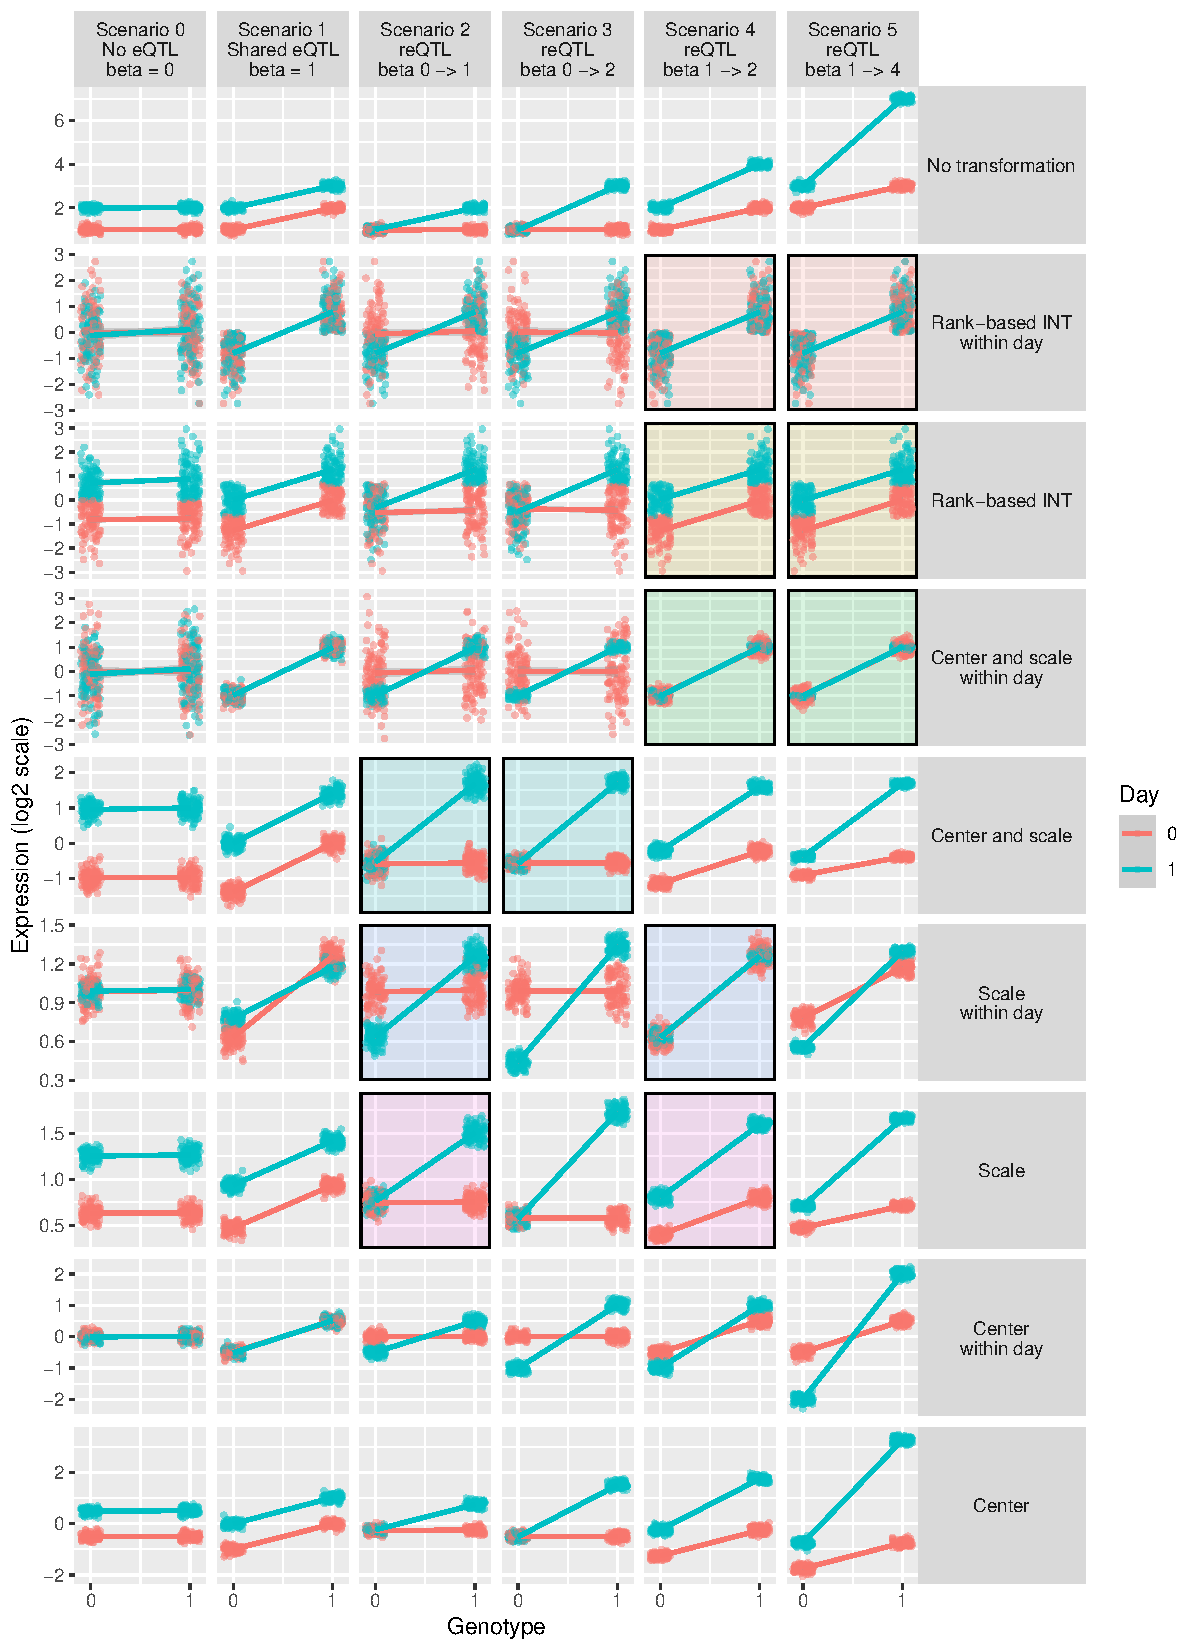
\includegraphics[width=1.0\textwidth,page=1]{mainmatter/figures/chapter_03/simulate_expression_transforms.pdf}
    \caption{expression xforms}
    \label{fig:hird_eQTL_expressionTransform_sims}
\end{figure}

\subsection{Estimation of cell type abundance via expression deconvolution}
\todo{not technically deconv}

% Also, \gls{RNAseq} expression estimates are inherently compositional \url{https://www.ncbi.nlm.nih.gov/pubmed/29608657} \url{https://academic.oup.com/gigascience/article/8/9/giz107/5572529}.
As \gls{PBMC} samples are a mixture of immune cells, and a fixed input of RNA extracted from that mixture is used to estimate expression, estimates for genes that have cell type specific expression depend on the relative proportions of each cell type in each sample, which shift after Pandemrix vaccination\autocite{sobolev2016AdjuvantedInfluenzaH1N1Vaccination}.
\gls{eQTL} effects can also be cell type specific\todo{determine appropriate citations from existing refs in ch1}.
The effect of genotype on expression can be compared between multiple timepoints to call \glspl{reQTL} as genotype can be assumed to stay constant, 
but changes in cell type abundance confound this by modifying both expression and the effect of genotype on expression.
Immune cell abundance also varies naturally between healthy individuals (\url{https://www.sciencedirect.com/science/article/pii/S0092867414015906?via%3Dihub}, \url{https://www.nature.com/articles/nri.2016.125}), so it is important to model these effects even at baseline.

Cell type abundance directly measured via \gls{FACS} are only available for a small subset of \gls{HIRD} individuals,
so I used expression deconvolution as an alternative to derive cell type abundances from bulk expression data for use in \gls{eQTL} modelling\autocite{davenport2018DiscoveringVivoCytokineeQTL,kim-hellmuth2019CellTypeSpecific}.
\todo{deconv returns an aggregate measure, so should not confound results for any one gene}
% https://github.com/dviraran/xCell
%
% xCell uses the expression levels ranking and not the actual values, thus
% normalization does not have an effect, however normalizing to gene length is
% required.
%
% Importantly, xCell performs best with heterogenous dataset. Thus it is
% recommended to use all data combined in one run, and not break down to pieces
% (especially not cases and control in different runs).  xCell uses the
% variability among the samples for the linear transformation. xCell will only
% function with heterogenous mixtures. If there is no variability between the
% samples, xCell will not identify any signal. As noted above, it is highly
% recommended to use all data combined in one run. Failing to do so will again
% inevitably make xCell's results false.
%
% xCell produces enrichment scores, not percentages. It is not a deconvolution
% method, but an enrichment method. That means that the main usage is for
% comparing across samples, not across cell types. xCell does an attempt to make
% the scores resemble percentages, but it is a hard problem, and is very platform
% and experiment specific. We have made some tests to compare the ability of
% xCell for cross-cell types analysis, and found that it generally performed
% better in that than other methods (on limited and comparable cell types), but
% this type of analysis should be performed carefully.  Regarding this issue,
% scaling the scores by samples is extremely dangerous and will inevitably will
% result in false interpretations.
I selected the \texttt{xCell} method, which previously been shown to outperform other deconvolution methods for cell type specific \gls{eQTL} mapping in blood\autocite{kim-hellmuth2019CellTypeSpecific}
\texttt{xCell} computes enrichment scores based on the expression ranks of approximately 10000 signature genes derived from purified cell types,
works for both array and \gls{RNAseq} expression data,
and implements \enquote{spillover compensation} to reduce dependency of estimates between related cell types\autocite{aran2017XCellDigitallyPortraying}.
%
% The spillover compensation step may over compensate, thus it is always better
% to run xCell with a list of cell types that are expected to be in the mixture.
% The names of cell types in this list must be a subset of the cell types that
% are inferred by xCell.
%
\texttt{xCell} was originally developed for tumor samples, so many of the built-in cell types are not relevant to this study.
% See 2019-11-14 log
% https://link.springer.com/chapter/10.1007/978-3-319-16104-4_15
% https://www.nature.com/articles/s41588-018-0089-9
% www.blueprint-epigenome.eu/index.cfm?p=7BCEDA45-EC73-3496-2C823D929DD423DB
Reviewing the literature to find which broad classes of peripheral blood cell types might be commonly-expected the \gls{PBMC} compartment\autocite{davenport2018DiscoveringVivoCytokineeQTL},
I selected 7/64 of the built-in cell types: 'CD4+ T-cells', 'CD8+ T-cells', 'B-cells', 'Plasma cells', NK cells, Monocytes and DCs.
% /nfs/users/nfs_b/bb9/workspace/phd/output/hird/rnaseq/4_de/array/array_data_setup.y.filtered.MaxMean.combat.rds
% and /nfs/users/nfs_b/bb9/workspace/phd/output/hird/rnaseq/4_de/array/array_data_setup.sample.metadata.merged.rds
\gls{RNAseq} and array expression data from sections\todo{link in preproc sections ch2} were processed separately; the large batch effect present in the array expression was first removed using ComBat.
Finally, enrichment scores were standardised, so that score of zero estimates the average abundance of that cell type across all timepoints (\autoref{fig:hird_xCell_scores_heatmap_array, fig:hird_xCell_scores_heatmap_rnaseq}).

\begin{figure}
    \centering
    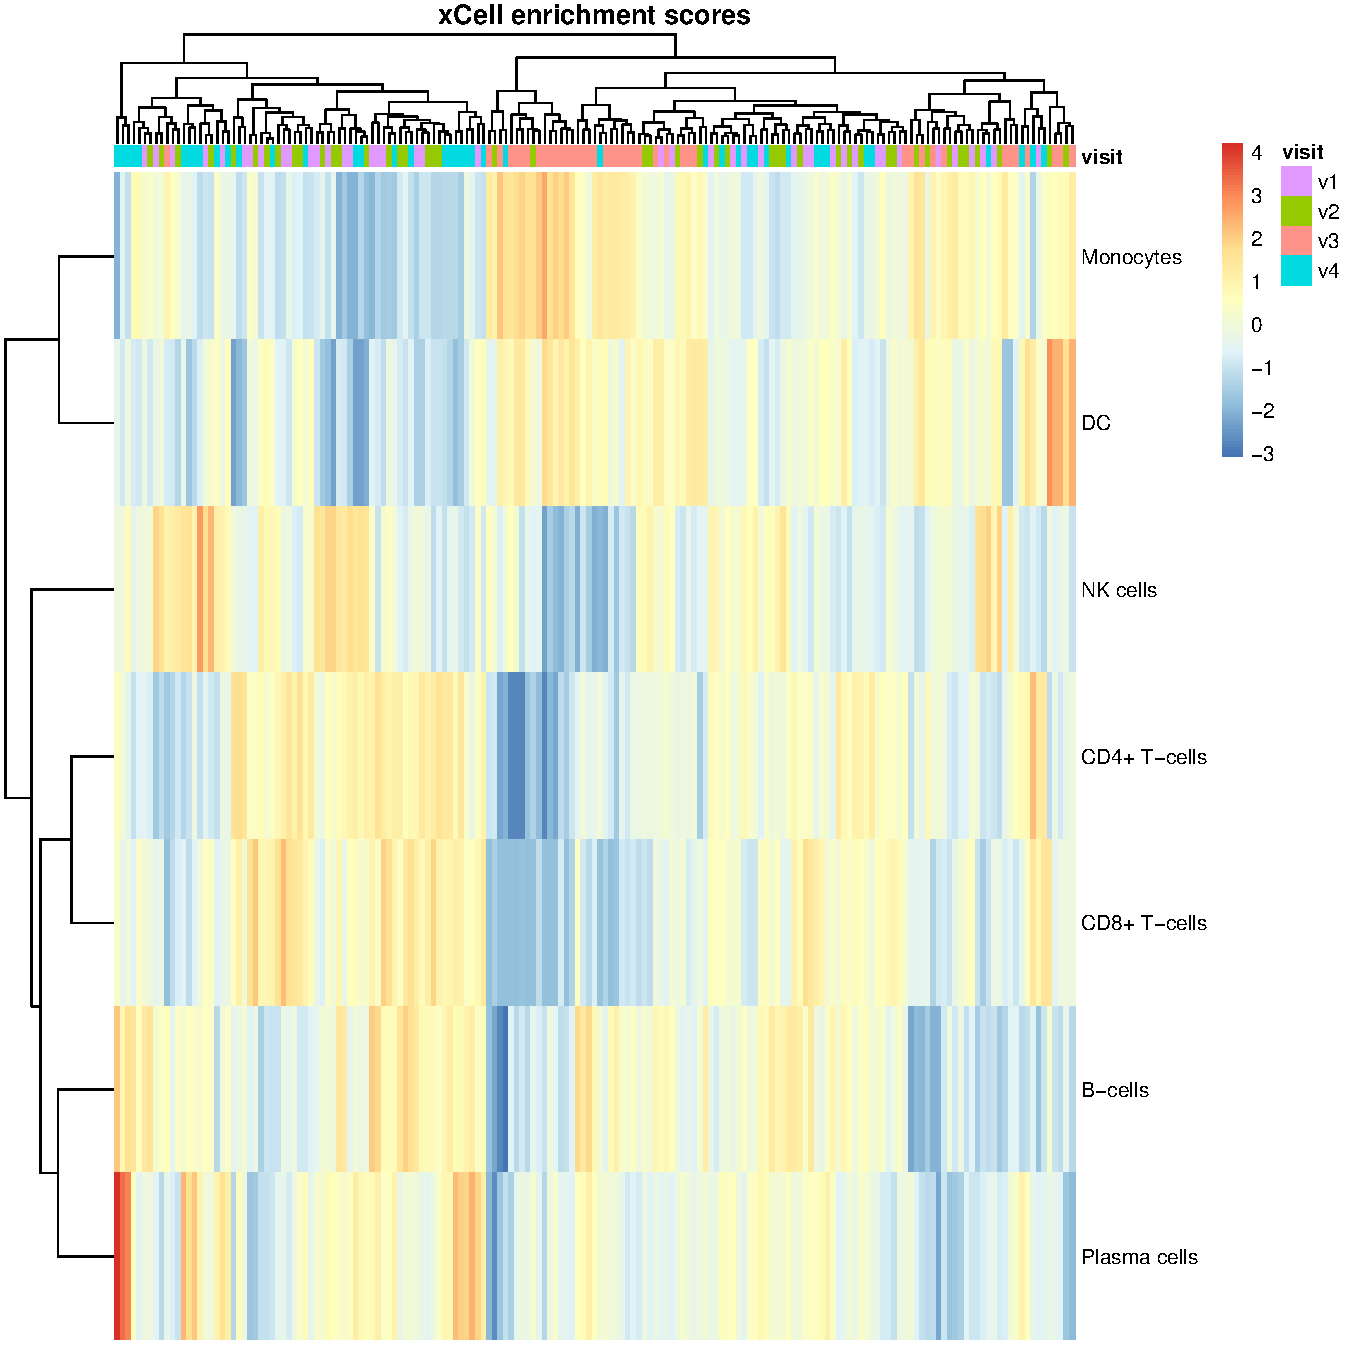
\includegraphics[width=1.0\textwidth,page=1]{mainmatter/figures/chapter_03/get_xCell_estimates.dataset_array.plots.pdf}
    \caption{xCell enrichment scores in array data}
    \label{fig:hird_xCell_scores_heatmap_array}
\end{figure}

\begin{figure}
    \centering
    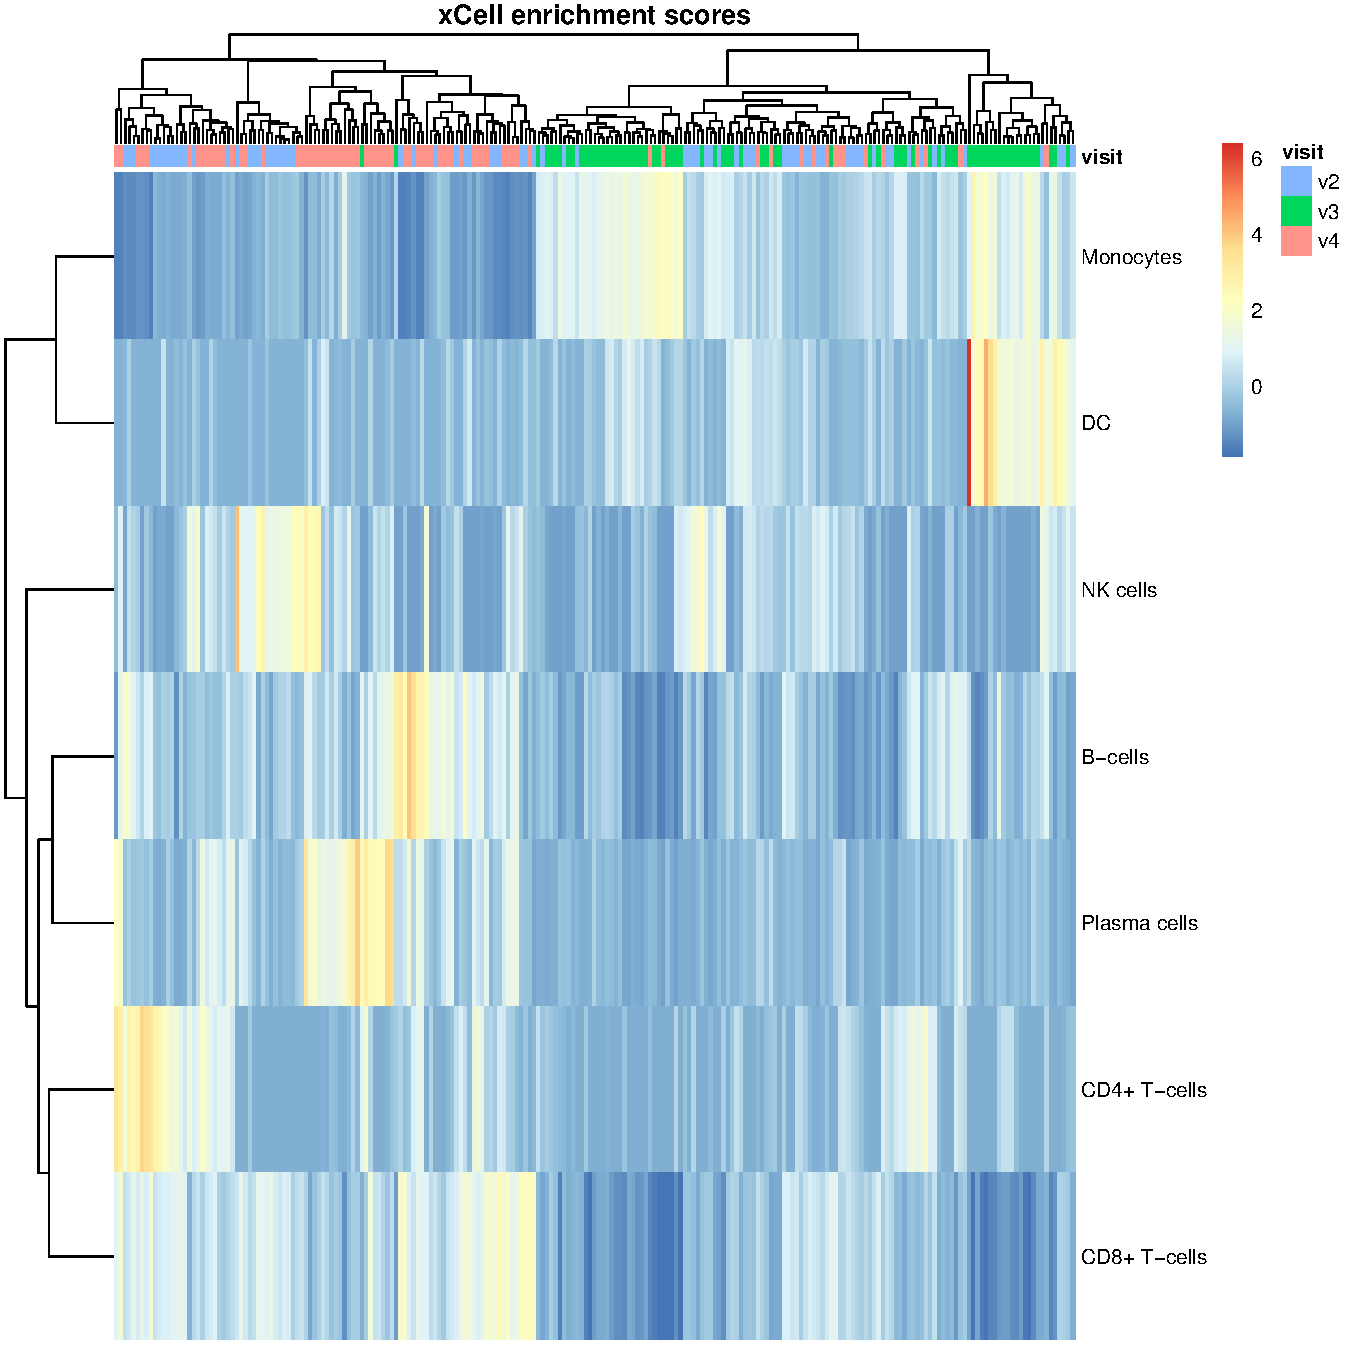
\includegraphics[width=1.0\textwidth,page=1]{mainmatter/figures/chapter_03/get_xCell_estimates.dataset_rnaseq.plots.pdf}
    \caption{xCell enrichment scores in rnaseq data}
    \label{fig:hird_xCell_scores_heatmap_rnaseq}
\end{figure}

As with actual cell type abundances, the enrichment scores are correlated.
Multicollinearity will be a problem for interpreting effect size estimates when these scores are used as covariates downstream.
To prune the number of scores, I performed a \gls{PCA} of the cell type scores across samples,
determined the number of principal components that exceed the eigenvalues-greater-than-one rule of thumb\url{doi 10.22237/jmasm/1162353960},
then selected only one cell type with high contribution to each of those components.
In both array and \gls{RNAseq} datasets, the selected cell types were monocytes, \gls{NK} cells, and plasma cells (\autoref{fig:hird_xCell_cos2}).
The choice to use actual enrichment scores over principal components directly as covariates is a sacrifice of orthogonality for interpretability.

% var$contrib: contains the contributions (in percentage) of the variables to the
% principal components. The contribution of a variable (var) to a given principal
% component is (in percentage) : (var.cos2 * 100) / (total cos2 of the
% component).
\begin{figure}
    \centering
    \begin{subfigure}[b]{0.49\textwidth}
        \centering
        \includegraphics[width=1.0\textwidth,page=8]{mainmatter/figures/chapter_03/get_xCell_estimates.dataset_array.plots.pdf}
        \caption{array}
    \end{subfigure}%
    \hfill%
    \begin{subfigure}[b]{0.49\textwidth}
        \centering
        \includegraphics[width=1.0\textwidth,page=8]{mainmatter/figures/chapter_03/get_xCell_estimates.dataset_rnaseq.plots.pdf}
        \caption{rnaseq}
    \end{subfigure}%
    \caption{xCell cos2 contributions}
    \label{fig:hird_xCell_cos2}
\end{figure}

Scores were validated against \gls{FACS} measurements in the subset of individuals that had them.
Depending on each panel's gating strategy, the \gls{FACS} data were in mixed units of both absolute and percentage cell counts.
A rank-based \gls{INT} was applied within each panel and cell type (\autocite{astle2016AllelicLandscapeHuman} takes a similar approach for cell abundance data using a quantile-based \gls{INT}).
% Also in phenome scan PHEASANT https://www.biorxiv.org/content/biorxiv/early/2017/02/26/111500.full.pdf
%
% missForest is a nonparametric imputation method for basically any kind of data.
% It can cope with mixed-type of variables, nonlinear relations, complex
% interactions and high dimensionality(p>>n). It only requires the observation
% (i.e. the rows of the data frame supplied to the function) to be pairwise independent.
Missing values were imputed with \texttt{missForest}, a random forest imputation method suitable for high-dimensional data where p >> n.
% NOTE:
% Why impute for cell counts but not for expression data?
% - expression matrices are mostly complete, and we only exclude genes based on low expression in RNAseq
% - we cannot drop whole FACS panels so easily like we can drop genes
Although the increase in xCell score for monocytes at day 1 and plasma cells at day 7 reflect the increases in these cell types observed by\autocite{sobolev2016AdjuvantedInfluenzaH1N1Vaccination}, overall correlation between xCell and \gls{FACS} was weak (\autoref{fig:hird_xCell_vs_FACS}).
Weighing the downside of having imperfect estimates of cell type abundance against the downsides of not accounting for abundance, or excluding samples without \gls{FACS} measures, I chose continue the analysis using the xCell scores.

\begin{figure}
    \centering
    \begin{subfigure}[b]{0.43\textwidth}
        \centering
        \includegraphics[width=1.0\textwidth,page=6]{mainmatter/figures/chapter_03/validate_xCell_estimates.cell_type_pairs.pdf}
        \caption{mono}
    \end{subfigure}%
    \vspace{1em}\vfill%
    \begin{subfigure}[b]{0.43\textwidth}
        \centering
        \includegraphics[width=1.0\textwidth,page=3]{mainmatter/figures/chapter_03/validate_xCell_estimates.cell_type_pairs.pdf}
        \caption{nk}
    \end{subfigure}%
    \vspace{1em}\vfill%
    \begin{subfigure}[b]{0.43\textwidth}
        \centering
        \includegraphics[width=1.0\textwidth,page=2]{mainmatter/figures/chapter_03/validate_xCell_estimates.cell_type_pairs.pdf}
        \caption{plasma}
    \end{subfigure}%
    \caption{xCell vs facs int}
    \label{fig:hird_xCell_vs_FACS}
\end{figure}

\subsection{Finding hidden confounders using factor analysis}

% If RANKINT, why RANKINT before PEER?
%
% Are your covariates under control? How normalization can re-introduce covariate effects
% https://www.ncbi.nlm.nih.gov/pubmed/29706643
% "Many statistical tests rely on the assumption that the residuals of a model are normally distributed [1]. In genetic analyses of complex traits, the normality of residuals is largely determined by the normality of the dependent variable (phenotype) due to the very small effect size of individual genetic variants [2]. However, many traits do not follow a normal distribution."
% "applying rank-based INT to the dependent variable residuals after regressing out covariates re-introduces a linear correlation between the dependent variable and covariates, increasing type-I errors and reducing power."

% 2.	Infer global confounders by detecting hidden factors affecting expression with PEER
% 2.1.	“batch effects and other global confounders reduce the power to find expression quantitative trait loci”
% 2.1.1.	“We assume that these variables have a broad influence, and thus each of them has an effect size for every gene.”
% 2.1.2.	“The learned variables can be constrained to affect known sets of genes via a prior connectivity matrix. By default, with no prior connectivity given, they are assumed to be global and to affect large fractions of all genes“
% 2.1.3.	Note that due to this assumption: “If large trans hotspots are dominating, associations may get erroneously explained away as confounding factors”
% 2.2.	Round input expression to integer counts
% 2.2.1.	Input is y: the scaledTPM (TPM's scaled up to library size) from tximport.
% 2.3.	Normalise for library size and variance stabilize with varianceStabilizingTransformation from DESeq2 (recommended in PEER paper)
% 2.3.1.	Vst is like a souped up log: “In all cases, the transformation is scaled such that for large counts, it becomes asymptotically (for large values) equal to the logarithm to base 2 of normalized counts.”
% 2.3.2.	Note we cannot use voom-ed expressions from the DGE pipeline, as there are some samples missing due to lack of Ab titre data
% 2.3.3.	Do not blind the transformation to experimental design matrix: “If many of genes have large differences in counts due to the experimental design, it is important to set blind=FALSE for downstream analysis.”
% 2.3.4.	Here we use a simple design matrix of groups defined by all combos of day x R/NR
% 2.4.	Run PEER by timepoint
% 2.4.1.	Match GTeX pipeline: https://github.com/broadinstitute/gtex-pipeline/tree/63b13b8ced25cf8ab8e7a26f40a495e523630a9b/qtl , with some modifications.
% 2.4.1.1.	Note this pipeline uses quantile normalized, rank INT transformed expression, as PEER input
% 2.4.2.	Quantile normalize the samples with preprocessCore::normalize.quantiles
% 2.4.2.1.	Causes the expressions of the samples to have the same empirical distribution
% 2.4.2.2.	i.e. the the highest expression in each sample is set to the mean of the highest values of all samples, and in the case of no tied values, each sample’s expressions becomes a permutation of each other sample’s
% 2.4.3.	Standardize expression of each gene with Rank-Based Inverse Normal Transformation
% 2.4.3.1.	i.e. rank the expressions of a gene, then replace with values from the standard normal e.g. > rank.based.INT(1:5, c=3/8): [1] -1.1797611 -0.4972006  0.0000000  0.4972006  1.1797611
% 2.4.4.	Setup and run PEER
% 2.4.4.1.	Allow up to 10k iterations, start with n.samples/4 PEER factors
% 2.4.4.2.	One can include known covariates. We don’t, as it causes weird things like PEER factors not being sorted in descending relevance
% 2.4.4.2.1.	~ 1 + batch + rna.conc + Gender + Age.at.vaccination..years. + PC1.imputed + PC2.imputed + PC3.imputed + PC4.imputed
% 2.4.4.2.2.	Note this includes an intercept that represents the mean expression
%
% Also interesting:
% PANAMA/LIMMI, by PEER authors
% Detecting regulatory gene–environment interactions with unmeasured environmental factors
%
Apart from cell type abundance, a myriad of other unmeasured variables also contribute to expression variation.
Hidden determinants of expression variation were learnt using \texttt{PEER}\autocite{stegle2012UsingProbabilisticEstimation}.
As recommended by \autocite{stegle2012UsingProbabilisticEstimation}, between-sample normalisation and variance stabilisation \gls{RNAseq} data was performed using \texttt{DESeq2::vsn},
then ComBat was applied to first merge array and \gls{RNAseq} data into a single log scale expression matrix per timepoint, treating the two array batches and three \gls{RNAseq} library prep pools as known batch effects.
% (e.g., by introducing principal components of the genotype data), is not included in the model, and it may be recapitulated in the inferred factors.
Given known covariates (intercept, sex, four genotype \glspl{PC} from section \todo{} representing ancestry, and the three xCell scores estimated above),
PEER estimates additional hidden factors that explain variation in expression matrix.
Factors are assumed to be unmeasured confounders that have global effects on a large fraction of genes, 
whereas a cis-\gls{eQTL} will typically only have local effects, so factors should not interfere with the genotype term for the purposes of cis-\gls{eQTL} mapping,
but should soak up some of residual variation, hence improving power to detect cis-\glspl{eQTL}.
The analysis was run per timepoint, otherwise global changes in expression between timepoints induced by the vaccine would be recapitulated as factors.

Correlating the estimated factors to a larger set of known covariates reveals many correlations with xCell estimates, indicating that cell type abundance does indeed have substantial global effects on the expression matrix.
There is little correlation with known array or \gls{RNAseq} batch effects, indicating ComBat did an adequate job of removing batch- and platform-dependent global effects on expression (\autoref{fig:hird_peer_corMatrix_v2_mega}).
Note that I did not leave this adjustment for PEER to perform, as ComBat estimates centering and scaling factors per gene to adjust for batch effects, whereas the use of PEER factors represent a mean-only adjustment, which given the severity of the batch effect in this dataset (e \autoref{fig:hird_expression_pcs}), may be insufficient\autocite{zhang2018AlternativeEmpiricalBayes}.

\begin{figure}
    \centering
    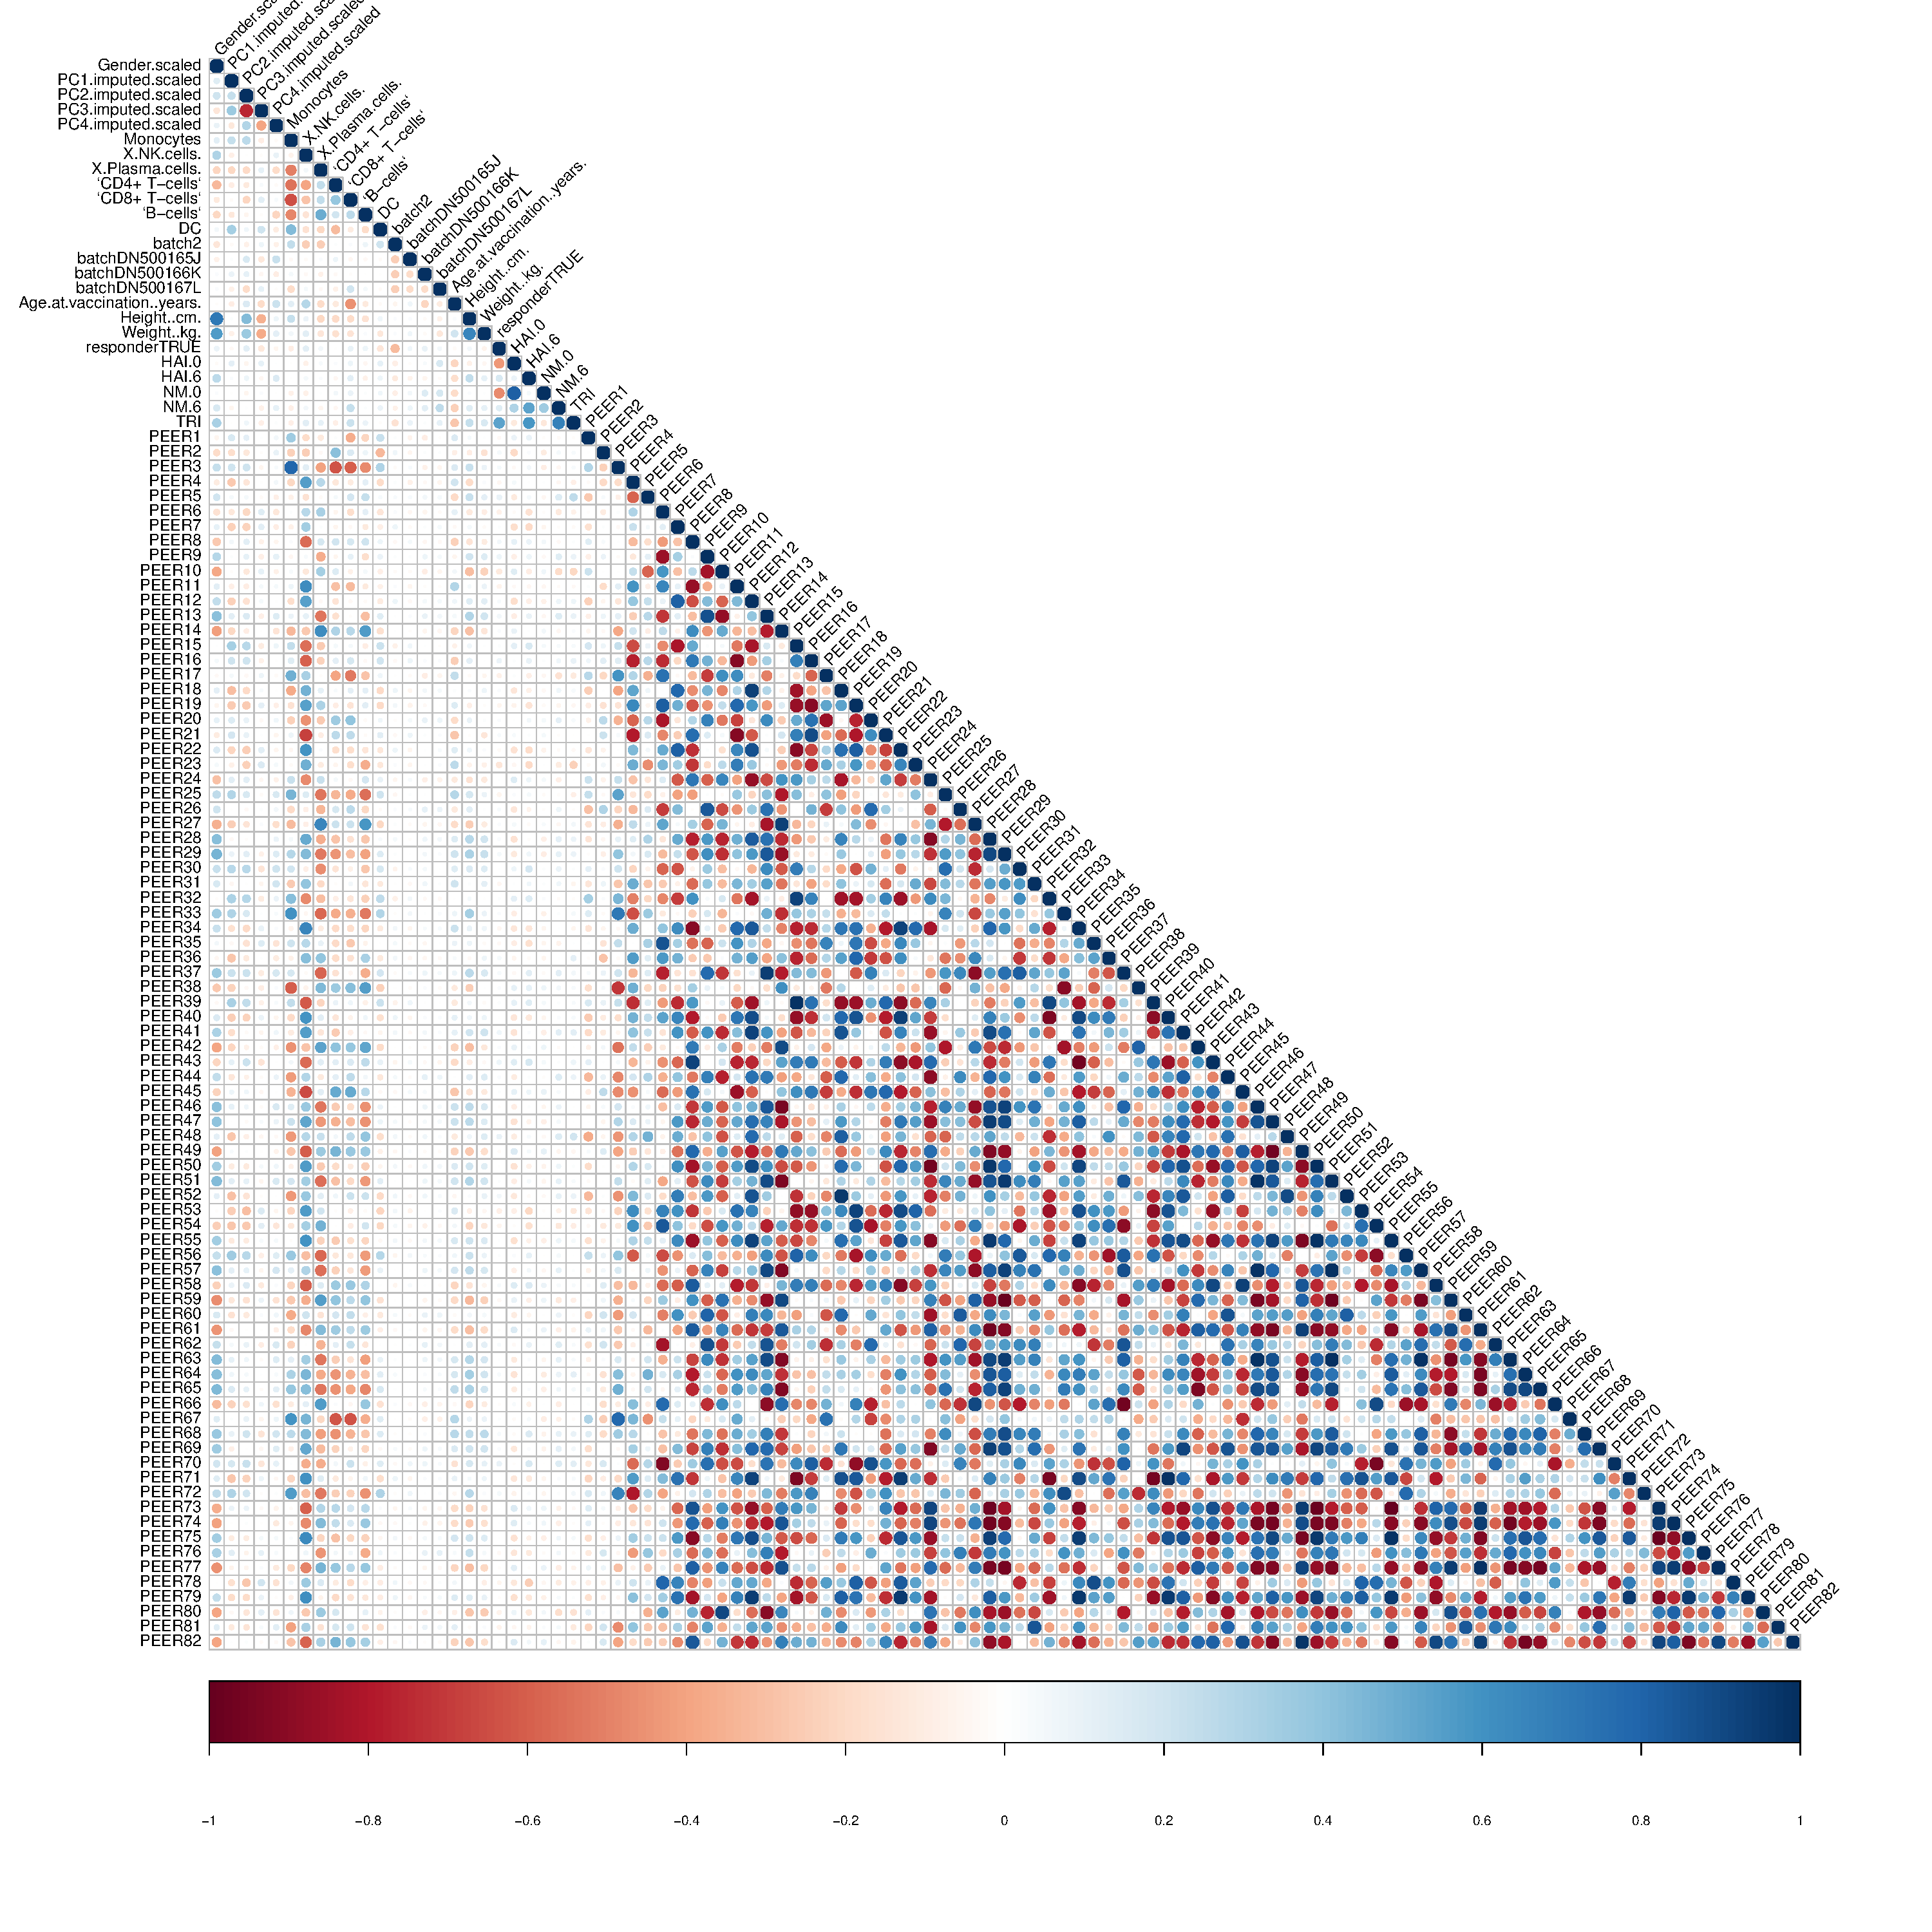
\includegraphics[width=1.0\textwidth,page=1]{mainmatter/figures/chapter_03/peer_mega/peer.factor_cor_matrix.v2.pdf}
    \caption{Note that PEER factors are not constrained to be orthogonal, so correlations to the provided known factors are expected.}
    \label{fig:hird_peer_corMatrix_v2_mega}
\end{figure}

\subsection{\glsfmtshort{eQTL} mapping per timepoint}

% 2.5.	Preprocess genotypes for limix
% 2.5.1.	Convert MAF filtered VCF -> 012 -> hdf5 format
% 2.5.1.1.	Do this for both strict 012 and continuous dosages
% 2.5.2.	Also convert 012 -> matrix eqtl SNP matrix format
% 2.5.2.1.	For eigenMT
% 2.5.3.	Parse out snpinfo and snplocs from VCFs
% 2.5.3.1.	Snpinfo for snp ids, for limix
% 2.5.3.2.	Snplocs for snp positions, and eigenMT
% 2.6.	Map eQTLs using limix 2.0, per timepoint
% 2.6.1.	Map cis-eQTLs within +- 1Mb of the gene start
% 2.6.1.1.	Phenotypes: per timepoint normalised input.expr from PEER script
% 2.6.1.2.	Covariates: sex, batch, 4 genotype PCs, 4 PEER factors
% 2.6.1.3.	Genotypes: MAF > 0.10 (in whole 169 individuals)
% 2.6.1.4.	Kinship: from LDAK, leave-one-chrom-out
% 2.6.2.	Output results in matrix eqtl-like output format
%
% For list of various methods considered, also see 2018-03-05, 2018-07-25, 2018-07-27 etc. in log
The performance of various software implementations of \glspl{LMM} specialised for genetic association studies are highly comparable; 
the specific choice of implementation can usually be made on the basis of computational efficiency\autocite{eu-ahsunthornwattana2014ComparisonMethodsAccount}.
I map \glspl{eQTL} within each timepoint using \texttt{LIMIX}\autocite{lippert2014LIMIXGeneticAnalysis}, which implements efficient univariate and multivariate \glspl{LMM} with one or more random effects.

Imputed genotype probabilities were converted to alternate allele dosages using bcftools (1.7-1-ge07034a).
Variants with sample \gls{AC} <= 15 within each timepoint were excluded.
% As is standard for imputation, we excluded all X-linked SNPs for the
% following reasons: (i) the X chromosome has to be treated differently from
% the autosomes; (ii) it cannot be predicted which allele is active on the X
% chromosome, (iii) testing males separately from females results in different
% sample sizes and power. Imputation of SNPs in the HapMap CEU population was
% performed using either MACH46 or IMPUTE47. All SNPs with a MAF <0.01 were
% excluded from analysis. In total, up to 2.11 million genotyped or imputed
% SNPs were analyzed.
X chromosome variants were excluded, as the number of copies differ between males and females, and X-inactivation makes it difficult to determine the active allele \url{https://www.nature.com/articles/ng.467},
% For example, an allele count of 1 in a female indi-cates a heterozygote
% genotype (one reference and onealternative allele), while a count of 1 in a
% male means only alternative allele exists and may cause more pro-found
% effects. The variance of the genetic effect may also differ between genders.
so sex-specific methods are required \url{http://www.biomedcentral.com/1471-2105/15/392}.

\todo{xchrom}
At each of 13126 autosomal genes, at all cis-variants within within +-1 Mb of the \gls{TSS}, I fit the following model to map \gls{eQTL}:
\begin{equation}
\begin{split}
Y = 1 + sex + \sum_{i=1}^{4}{PC_i} + \sum_{}^{3}{xCell} + \sum_{i=1}^{k}{PC_i} + G + \mathbf{u} + \epsilon
\end{split}
\end{equation}
\todo{lift proper vector notation from limix}

where \todo{}.

% note looc matrix for x chrom

PEER factors are automatically weighted such that the variance of factors tends to zero as more factors are estimated, 
hence continuing to add more and more factors as covariates will not continue to improve \gls{eQTL} detection power, and eventually the model degrees of freedom will be depleted.
To optimise k, the number of factors to include as covariates\footnote{I avoid the commonly-performed two-stage approach of treating PEER residuals as expression phenotypes, as the degrees of freedom seen downstream will be incorrect, which can have a substantial effect on estimates at this modest sample size\url{https://onlinelibrary.wiley.com/doi/abs/10.1002/gepi.20607}.}, 
Per-timepoint \gls{eQTL} mapping was performed just in chromosome 1, iteratively increasing the number of factors until the number of \glspl{eQTL} detected plateaus.
I settled on a final choice of k=10 factors for pre-vaccination, 5 factors for day 1, and 5 factors for day 7 (\autoref{fig:hird_neGenesvsPeerK}).

\begin{figure}
    \centering
    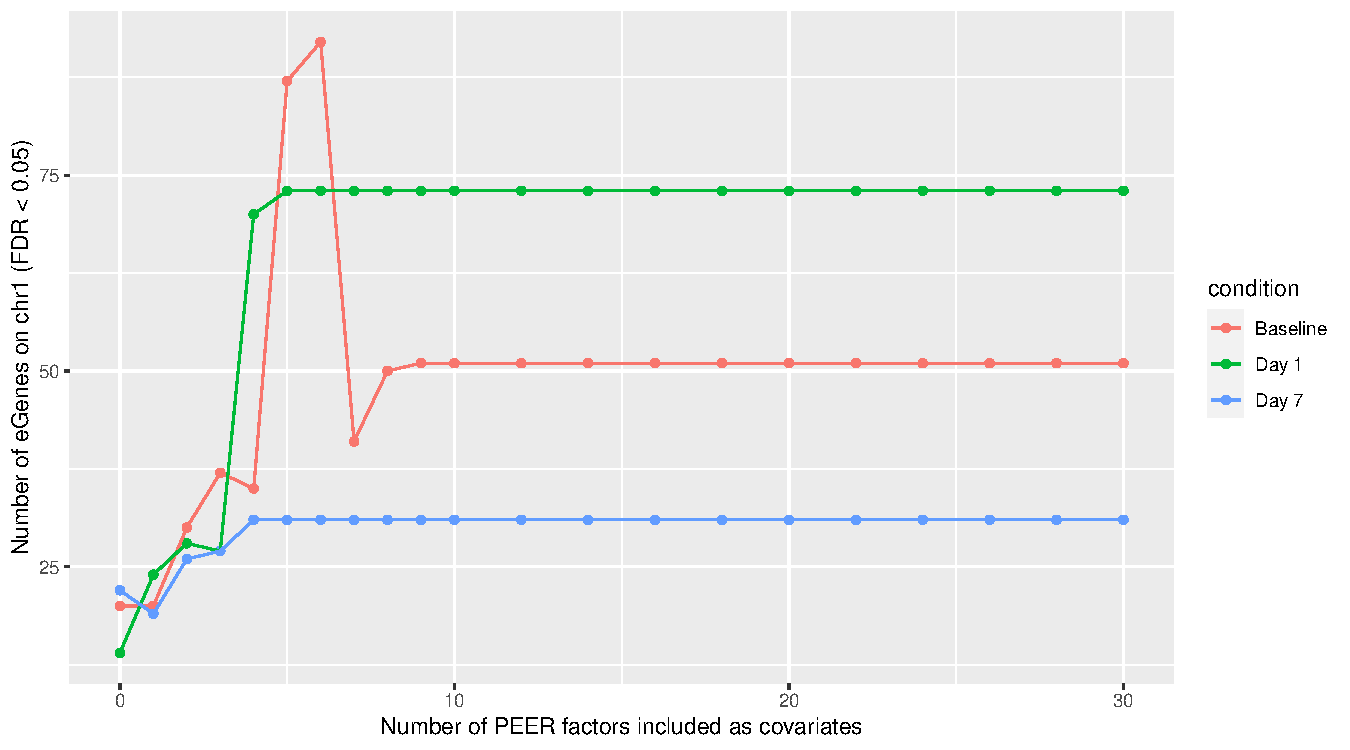
\includegraphics[width=1.0\textwidth,page=1]{mainmatter/figures/chapter_03/count_eGenes.signif_eGenes_vs_PEER_n.dataset_mega.chr_chr1.pdf}
    \caption{optimlise}
    \label{fig:hird_neGenesvsPeerK}
\end{figure}

\subsection{Joint \glsfmtshort{eQTL} analysis across timepoints}

\todo{snps only?}

% 2.10.	mashr
% 2.10.1.	Apply mashr to per-day meta-analysis beta/beta_ste results
Joint analysis was conducted with mashr, at 40197618 gene-variant pairs (tests) for which summary statistics from within timepoint mapping were available in all three timepoint conditions.

\glsfmtshort{eQTL}

The mashr model incorporates both canonical (e.g. the identity matrix) and data-driven covariance matrices to represent patterns of effects across conditions (in this case, 3 x 3 matrices).
Data-driven covariance matrices are derived by dimension reduction a strong subset of tests likely to have an effect in at least one condition.
I took the most significant variant per gene per condition, which ensures strong condition-specific effects are included (\autoref{fig:hird_mashr_strongSubset_Z_mega}, then further filtered to only nominally significant tests.

\begin{figure}
    \centering
    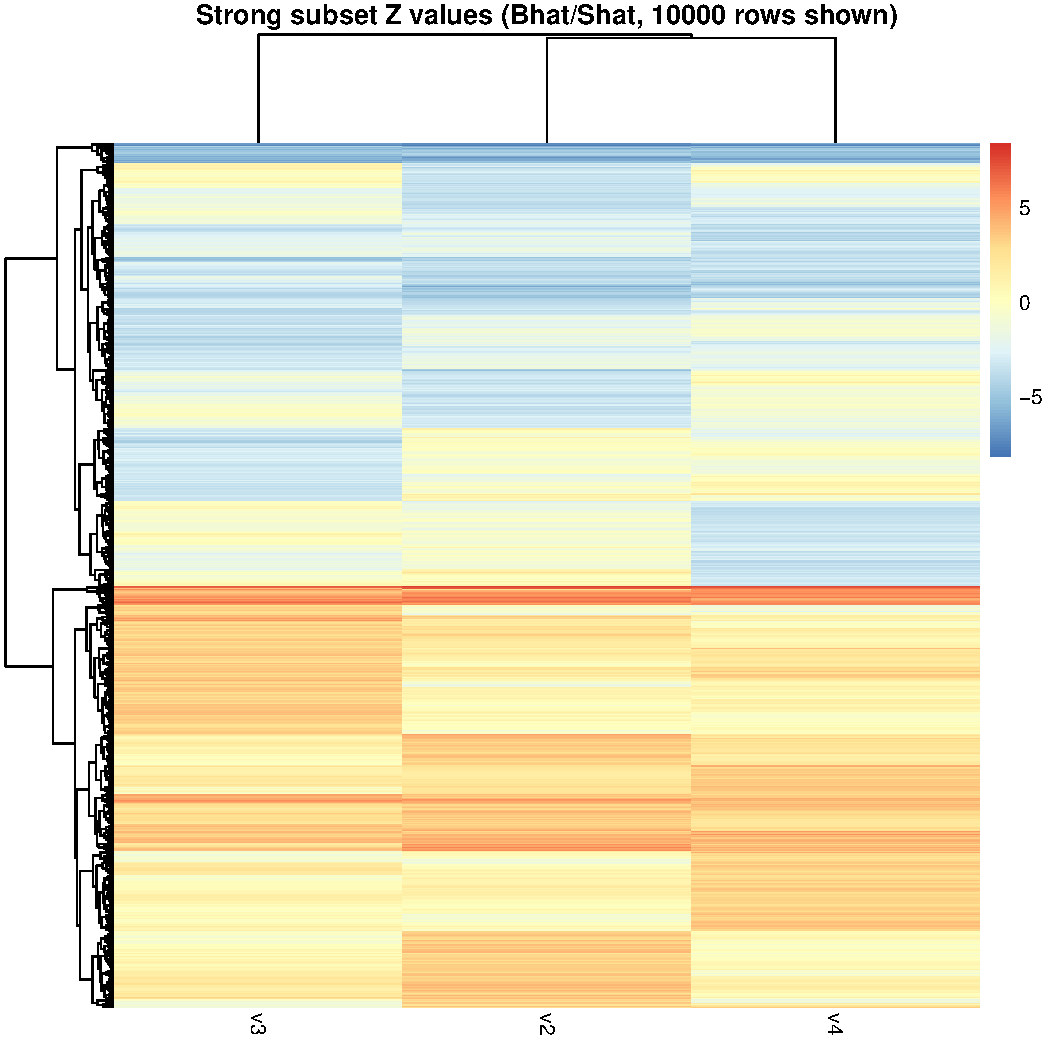
\includegraphics[width=1.0\textwidth,page=1]{mainmatter/figures/chapter_03/mash_mega/mashr.strong_subset_zval_heatmap.cisDist_1e6.sampleAcThresh_15.randomSubsetN_200000.pdf}
    % 45962 tests (including X)
    \caption{optimlise, sample 10k}
    \label{fig:hird_mashr_strongSubset_Z_mega}
\end{figure}

The mash model was trained on a random subset of 200000 tests, using the Exchangeable Z-scores model.
The correlation of null tests between conditions, important to account for due to the repeated measures structure of the data, was estimated using \software{mashr::estimate\_null\_correlation}.
The fitted model was used as a prior to compute posterior effects and standard errors for all tests through shrinkage.
% Stephens, M. (2016). False discovery rates: A new deal. Biostatistics, kxw041. https://doi.org/10.1093/biostatistics/kxw041
% analogous to a false discovery rate, but more stringent because it requires true discoveries to be not only nonzero, but also correctly signed.
%
% Also see:
% type s error rates for classical and bayesian single and multiple comparison procedures
% Why We (Usually) Don’t Have to Worry About Multiple Comparisons (2012)
% Beyond Power Calculations: Assessing Type S (Sign) and Type M (Magnitude) Errors (2014)
A condition-specific Bayesian measure of significance \gls{lfsr} is returned, which can be interpreted as the the probability given the data, that the declared sign of the effect is incorrect.
\todo{move lfsr to dge chapter}

\subsection{Defining shared and response eQTLs}

Many of the tested variants for each gene will be in high \gls{LD}.
% qtls.merged[, signif_rank := frank(qtls.merged, lfsr, -INFO, -MAF_sample, SNP_gene_TSS_dist, POS)]
To unambiguously select a lead \gls{eQTL} variant per gene tested, I selected the variant with the lowest lfsr in any condition, breaking ties by highest imputation INFO, highest \gls{MAF}, shortest distance to the \gls{TSS}.
Sharing was then evaluated for that gene-variant pair across all three conditions.

Thresholding on the lfsr is not appropriate for determining sharing, as the difference between significant and non-significant effect estimates in two conditions is not necessarily significant \url{http://www.stat.columbia.edu/~gelman/research/unpublished/signif3.pdf}.
% Not just use lfsr thresholds:
\autocite{urbut2018FlexibleStatisticalMethods} provides a heuristic that two effects are shared by magnitude if they have the same sign, and are also within a factor of 2 of one another.
Effects are also only compared if at least one of the two effects have lfsr < 0.05, to avoid sharing being driven by null effects.
% Also see:
%
% https://stats.stackexchange.com/questions/93540/testing-equality-of-coefficients-from-two-different-regressions
    % I found the key difference is whether the assumption that the error variance is the same or not.
% https://stats.stackexchange.com/questions/55501/test-a-significant-difference-between-two-slope-values
    % The classic (and more statistically powerful) way of testing this is to combine both datasets into a single regression model and then include the area as an interaction term. See, for example, here:
    % http://www.theanalysisfactor.com/compare-regression-coefficients/
    % This is "more ... powerful" only if more restrictive assumptions apply. In particular, it assumes homoscedasticity of error variances. Often one would not want to assume that (without additional justification) and therefore would use something like the Welch or Satterthwaite t-test. – whuber♦ Mar 30 '16 at 21:46
% https://andrewpwheeler.wordpress.com/2016/10/19/testing-the-equality-of-two-regression-coefficients/
    % Var(A-B) = Var(A) + Var(B) - 2*Cov(A,B)
    % NOTE: Assumes that Cov is 0, this is anticonservative when Cov is actually positive.
%
% See notes from 2018-10-11 on wald test, and comments on sharing_func in get sharing script
I combine this approach with the beta-comparison approach \url{https://psycnet.apa.org/record/1995-27766-001} \url{https://doi.org/10.1111/j.1745-9125.1998.tb01268.x} \autocite{schenker2001JudgingSignificanceDifferences} (applied to reQTLs by \autocite{kim-hellmuth2017GeneticRegulatoryEffects}), that also considers the standard error of both effects in the computation of a z score for the difference:

\begin{equation}
z = \frac{\beta_x - \beta_y}{\sqrt{\sigma_x^2 + \sigma_y^2 - 2\sigma^2(x, y)}}
\end{equation}

% Actually we can get:
% PosteriorCov
% Q x Q x J array of posterior covariance matrices, if the output_posterior_cov = TRUE.
The posterior pairwise covariance of effects for test $\sigma^2(x, y)$ is difficult to estimate, so here I assume $\sigma^2(x, y) = 0$, a generally conservative assumption if effects with opposite signs between conditions are generally rare.
Unlike a test for difference implemented using a genotype x condition interaction term in a joint regression model, homoscedasticity of errors is not assumed for all conditions \url{https://psycnet.apa.org/record/1995-27766-001}.
% Why can we use a Z test?
% Very similar to a Wald test. See 2018-10-11 log.
The z score can be compared to a standard normal to obtain a nominal Z-test p value for the difference in betas between each pair of conditions, at each gene's lead variant.

\subsection{Replication of eQTLs in a reference dataset}

To validate the \gls{eQTL} mapping approach, I estimate the replication of significant eQTLs in an independent reference.
Due to the lack of large sample size \gls{eQTL} maps specific to \gls{PBMC}, I use the GTEx v8 whole blood dataset as my reference dataset (n=670, 51.2\% eGene rate).
For lead variants called as significant in the \gls{HIRD} dataset at a given lfsr threshold, I lookup the nominal p value for that variant in GTEx (where the variant exists in both datasets).
I applied \software{qvalue::qvalue\_truncp} to estimate the proportion of those nominal p values that are null ($\pi_0$), the compute a measure of replication $\pi_1 = 1 - \pi_0$.

The mega-analysis has comparable replication rate for shared \glspl{eQTL} at moderately stringent \gls{lfsr} thresholds up to $10^{-5}$ (\autoref{fig:hird_eQTL_pi1vsGTExWholeBlood}).
Past this, as the $\pi_1$ procedure assumes a well-behaved p value distribution in $\left[0, 1\right]$, reliability declines due to the number of p values being too small\footnote{\url{https://github.com/StoreyLab/qvalue/pull/6\#commitcomment-26277751}}, or the maximum p value being too far from 1.
The numbers of \glspl{reQTL} were too low to assess replication using this method, and one might not expect them to replicate in a baseline dataset such as GTEx whole blood, especially for those \glspl{reQTL} significant only at post-vaccination timepoints.
As the mega-analysis has a higher eGene rate \todo{get exact numbers, roughly 50 vs 30pc} compared to the \gls{RNAseq}-only analysis, with similar replication,
I assume this represents is due to the power advantage from having larger a sample size, rather than technical effects from merging the expression data.

\begin{figure}
    \centering
    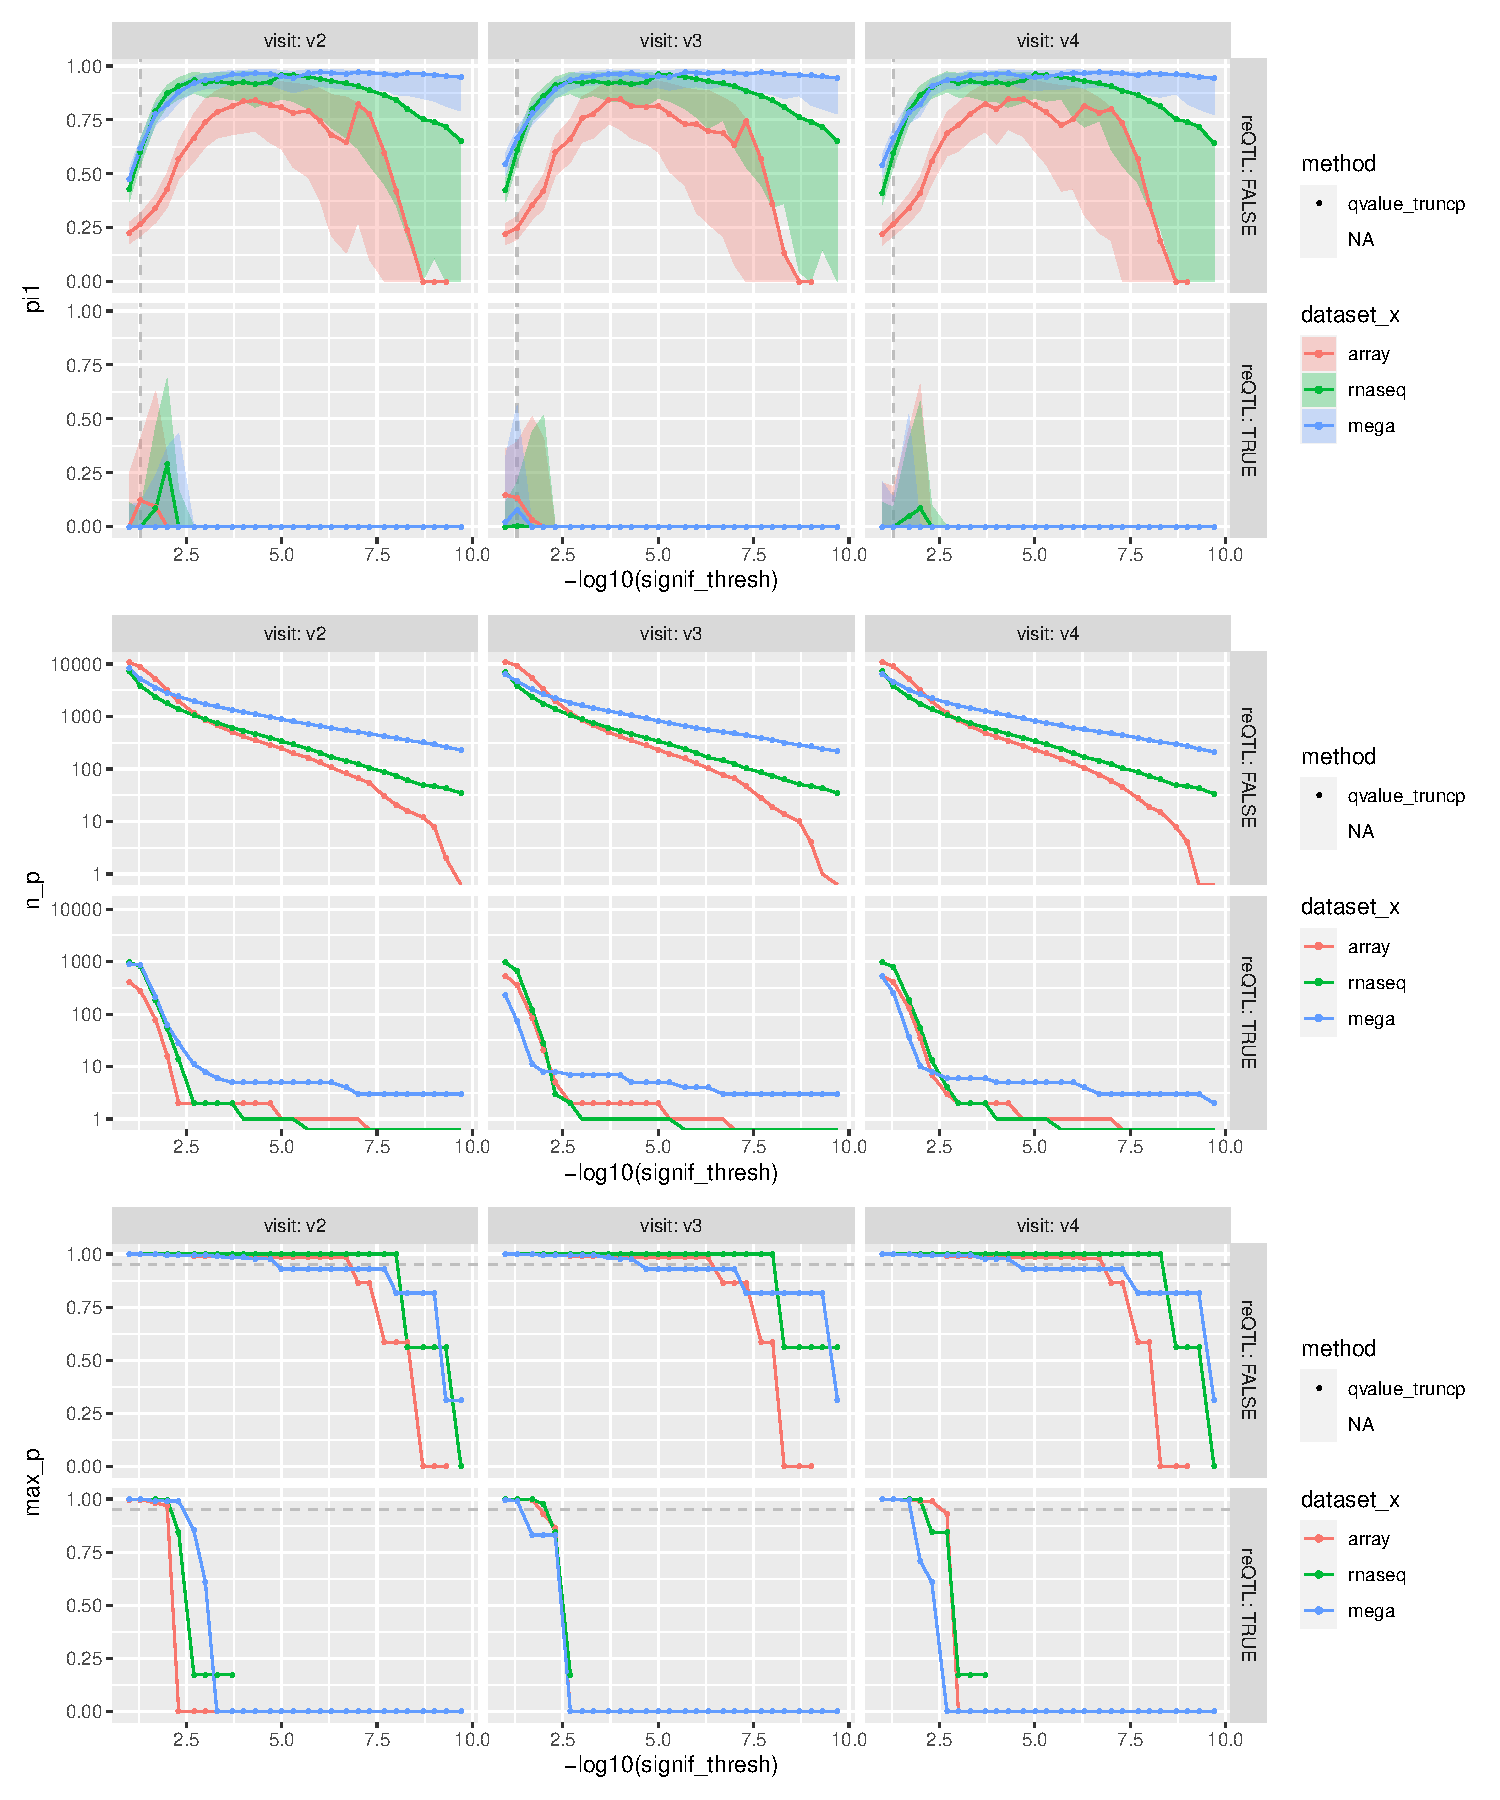
\includegraphics[width=1.0\textwidth,page=1]{mainmatter/figures/chapter_03/compute_pi1.pi1_by_thresholds.pdf}
    \caption{}
    \label{fig:hird_eQTL_pi1vsGTExWholeBlood}
\end{figure}


\subsection{Genotype interactions with non-timepoint predictors}

If the abundance of a particular cell type does truly modify the \gls{eQTL} effect, 
then an interaction term between genotype and cell type abundance is required, 
otherwise the slope of the \gls{eQTL} will represent an average across the abundance range for that cell type;
one can not \enquote*{} for this modification just by including the main effect for cell type abundance.

Given the modest sample size, I also use the two-step approach used by others\autocite{westra2015CellSpecificEQTL,peters2016InsightGenotypePhenotypeAssociations,kim-hellmuth2017GeneticRegulatoryEffects,davenport2018DiscoveringVivoCytokineeQTL},
where tests for interaction are only performed at a subset of tests, often the lead \gls{eQTL} variant for each gene.
% Unfortunately, there seems to be no consensus between these studies for controlling the interaction effect tests for multiple testing.
%
% Strange custom 5% FDR: westra2015CellSpecificEQTL
% Bonferroni: kim-hellmuth2017GeneticRegulatoryEffects
% Benjamini-Hochberg FDR: kim-hellmuth2017GeneticRegulatoryEffects
% Benjamini-Hochberg procedure, and a 0.15 FDR threshold: peters2016InsightGenotypePhenotypeAssociations
%
The key to the two-stage approach is that if the estimates for the interaction effect are sufficiently independent from the estimates of the main effect from main-effect only models,
the type I error can be controlled based on the number of interactions that are actually tested, rather the number of interactions that could have been tested for\autocite{kooperberg2008IncreasingPowerIdentifying,peters2016InsightGenotypePhenotypeAssociations}.
It is unclear whether this assumption holds, as the size of the main effect may contribute to power for detecting interaction effects.
As the main purpose of the interaction analyses is scanning for cell type effects at detected \glspl{reQTL},
I choose to test for interactions only at the lead \gls{eQTL} variant for each gene with a significant main \gls{eQTL},
then apply the \gls{BH} \gls{FDR} used by others\autocite{peters2016InsightGenotypePhenotypeAssociations,kim-hellmuth2017GeneticRegulatoryEffects}.

\gls{eQTL} models interactions between genotype and other predictors were fit using \software{lme4qtl}.
The model specification is as in \todo{above section}, with the addition of \todo{interactions with cel type/platform}.
Significance is assessed using the likelihood-ratio test versus the nested model with no interaction terms.

\section{Results}

\subsection{Mapping reQTLs to Pandemix vaccination}

Within each timepoint condition (day 0 pre-vaccination, day 1, and day 7), cis-\glspl{eQTL} ($\pm 1 \text{Mb}$ of the \gls{TSS}) were mapped using \software{LIMIX},
then joint analysis of effects was done using \software{mashr} to obtain posterior effect size and standard errors.
At \gls{lfsr} < 0.05, 6887/13570 genes (\percentage{0.5075166}) were eGenes (genes with a significant \gls{eQTL}) in at least one timepoint.
The most significant \gls{eQTL} variant across all timepoints was selected as the lead variant for each eGene.
\glspl{reQTL} were defined by comparing the effect size of this lead \gls{eQTL} between each pair of timepoints using beta-comparison approach.
Most \glspl{eQTL} were shared across timepoints; 1154/6887 (\percentage{0.1675621}) \glspl{eQTL} were classified as significant \glspl{reQTL} (nominal p difference < 0.05).

\autoref{fig:hird_eQTL_upset_mega} illustrates the difference between calling sharing using a significance threshold versus difference in betas approach.
For instance, day 0 was the timepoint with the largest number of eGenes, reflecting the larger sample size compared to other timepoints.
Although there are 1427 eGenes significant at only day 0, at 646/1427 eGenes, the effect size at day 0 does not differ significantly when compared to day 1 or day 7.
The most significant \glspl{eQTL} with the highest abs(z) in any timepoint are shared between timepoints, highlighting the power advantage for mapping shared effects granted by joint analysis.
Shared \glspl{eQTL} appear to be enriched close to the \gls{TSS}, whereas \glspl{reQTL} do not show this pattern.

\begin{figure}
    \centering
    % 
\includegraphics[width=1.0\textwidth,page=2]{mainmatter/figures/chapter_03/get_signif_qtls.upset.eGenes_sharing_no_ties_joint.dataset_mega.groups_v2_v3_v4.cisDist_1e6.sampleAcThresh_15.randomSubsetN_200000.signifThresh_0.05.pdf}
    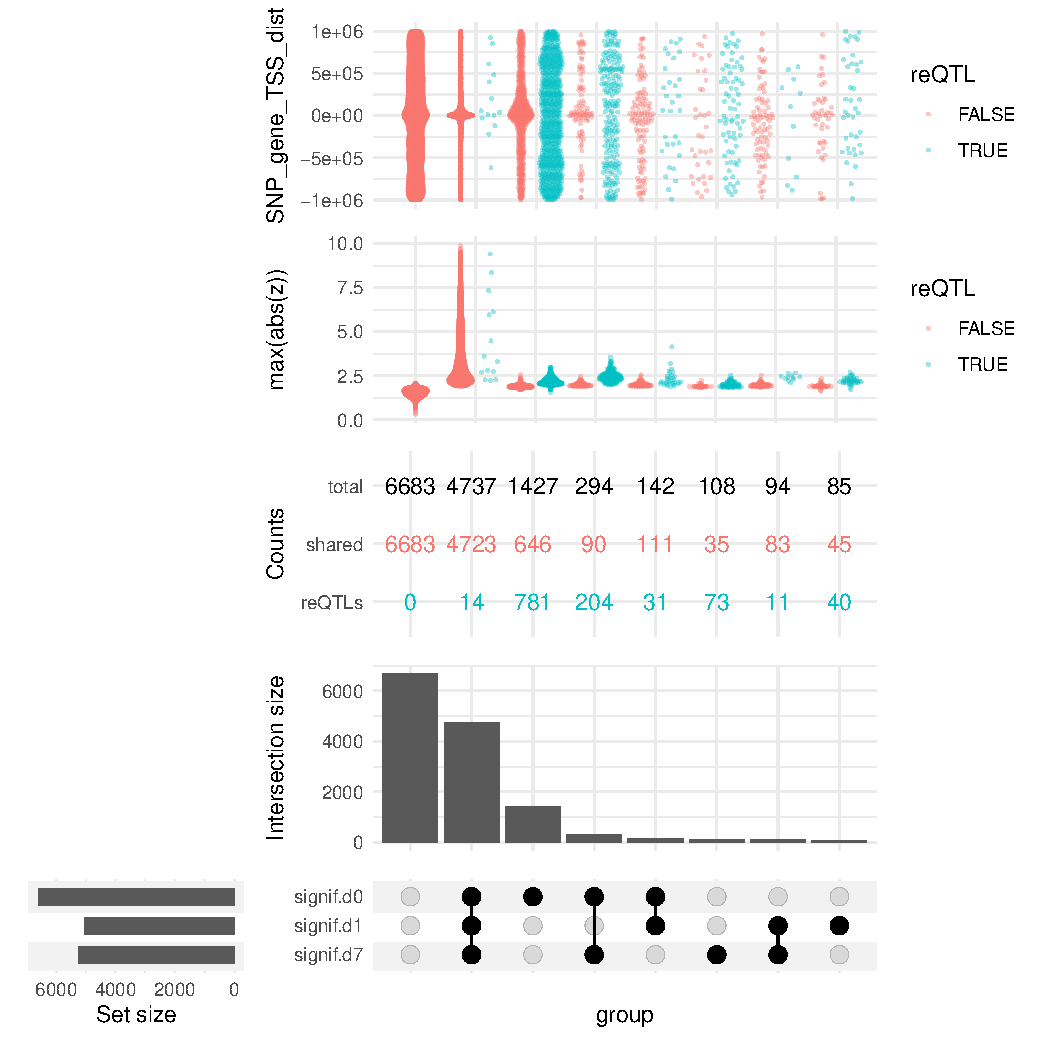
\includegraphics[width=1.0\textwidth]{mainmatter/figures/chapter_03/compare_dge_eqtl.upset.pdf}
    \caption{}
    \label{fig:hird_eQTL_upset_mega}
\end{figure}

% \begin{figure}
%     \centering
%     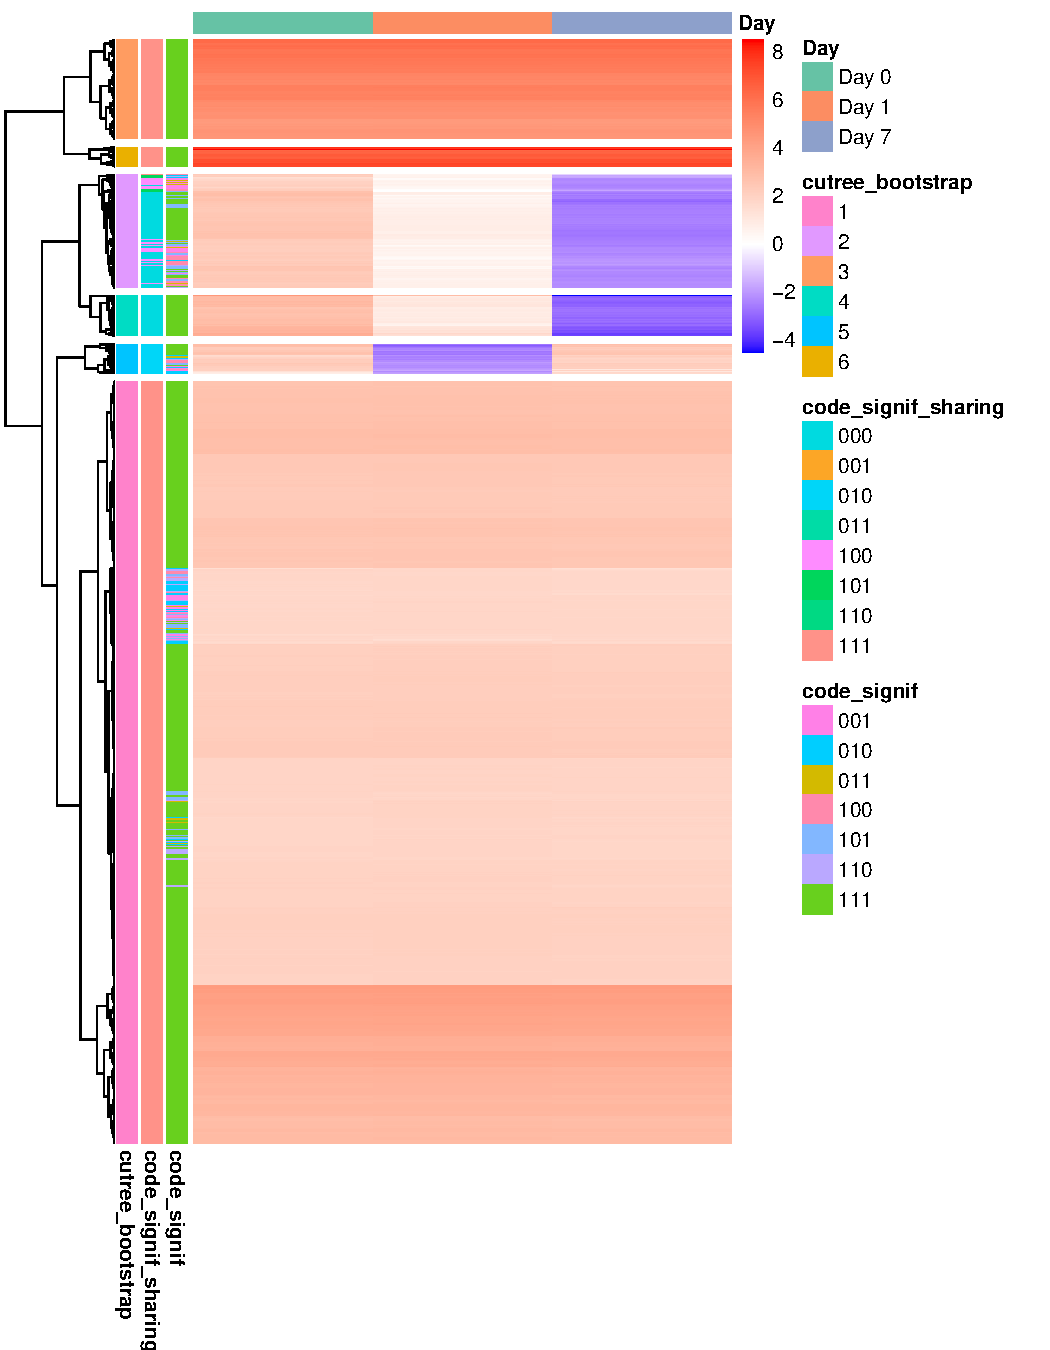
\includegraphics[width=1.0\textwidth,page=1]{mainmatter/figures/chapter_03/plot_dge_eqtl.heatmap_eqtl.pdf}
%     \caption{}
%     \label{fig:hird_eQTL_heatmap_mega}
% \end{figure}

\subsection{Characterising reQTLs post-vaccination}

I focus on \glspl{eQTL} that are significant post-vaccination, and explain more variation in expression post-vaccination, as the converse may be caused by greater power at day 0 rather than being a result of vaccine stimulation.
\todo{put pve formula in methods, include point that pve norms to var(y)}
Many of the \gls{reQTL} that satisfy this criteria have opposite effects pre- and post-vaccination (\autoref{fig:hird_eQTL_zSharing_vs_TSSdist_mega}).
Once again, shared \glspl{eQTL} are enriched close to the \gls{TSS}, and \glspl{reQTL} are distributed across the cis- window.
Gene set enrichment analysis on eGenes for these sets of \glspl{reQTL} at day 1 (68 eGenes) and day 7 (226 eGenes) did not detect any significant enrichments (\software{gprofiler2}, g:SCS adjusted p < 0.05).
%
% Possible Ranking metrics for ranked enrichments
%     PVE: prefers large maf and high betas since it squares the beta. even if the beta does not change so much. ignores sign.
%     beta:
%     p: ignores sign
%     Z score:

\begin{figure}
    \centering
    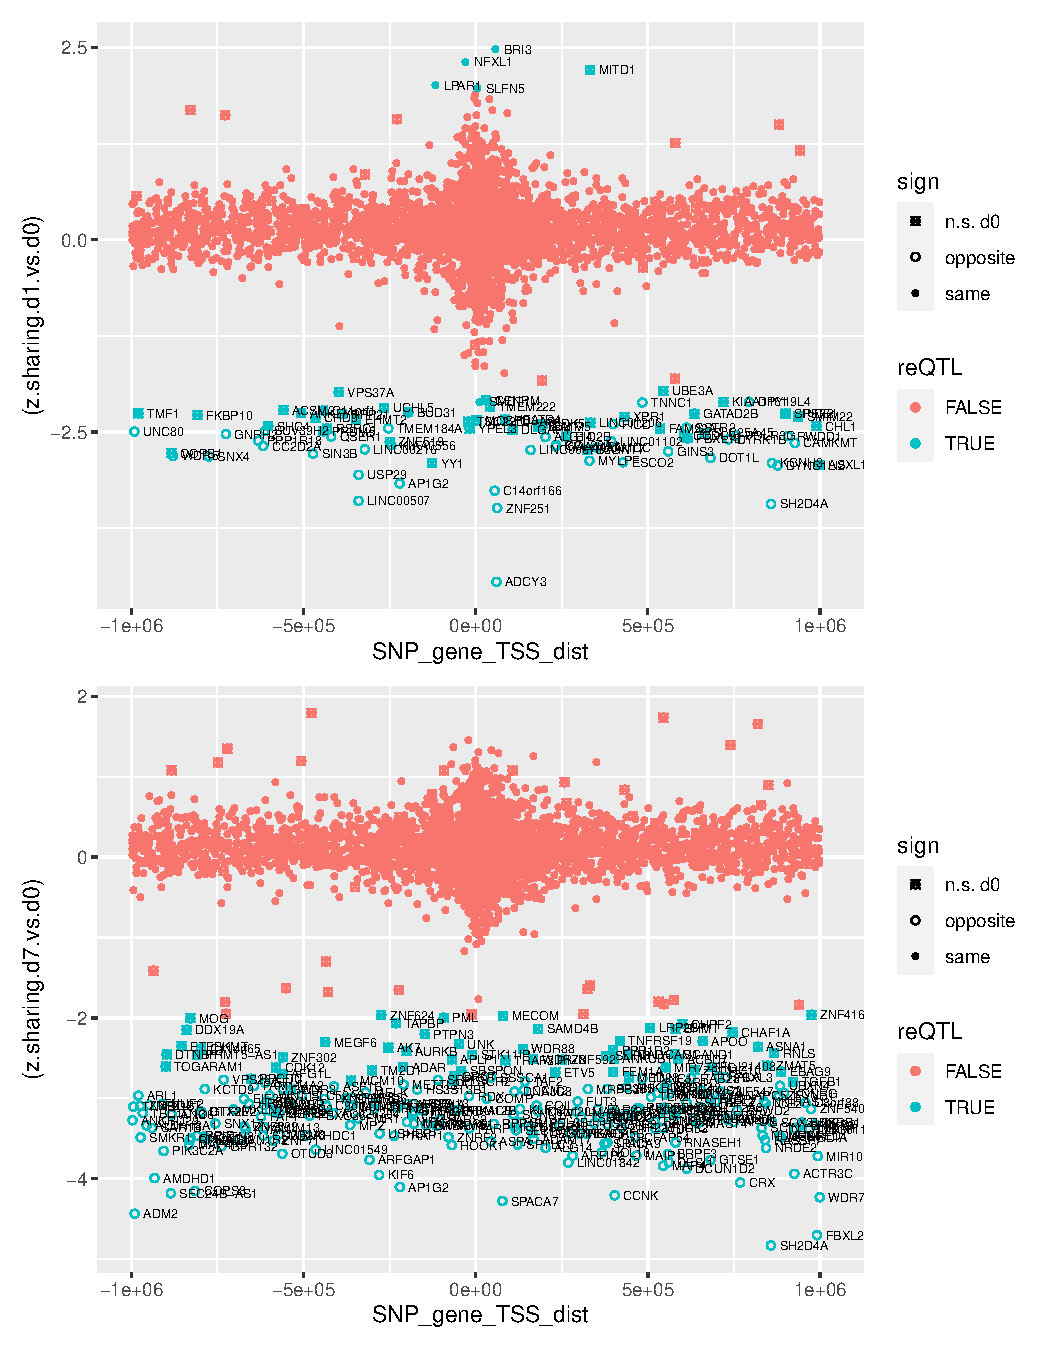
\includegraphics[width=1.0\textwidth]{mainmatter/figures/chapter_03/compare_dge_eqtl.z_sharing.vs.SNP_gene_TSS_dist.pdf}
    \caption{}
    \label{fig:hird_eQTL_zSharing_vs_TSSdist_mega}
\end{figure}

The strongest reQTL at day 1 was for \gene{ADCY3} (p difference = \num{8.676917e-06}, BH FDR = \num{0.1177458}),
where the \gls{reQTL} variant explained approximately \percentage{0.01862996} of expression variation at day 0, increasing to \percentage{0.14075782} at day 1 (\autoref{fig:hird_eQTL_ploteQTL_ADCY3}).
At day 7 the strongest \gls{reQTL} was at \gene{SH2D4A} (p difference = \num{1.369564e-06}, BH FDR = \num{0.01747935}).
Here, the \gls{reQTL} variant explained similar amounts of expression variation at day 0 (\percentage{0.08229266}) and day 7 (\percentage{0.08956865}), with opposite directions of effect (\autoref{fig:hird_eQTL_ploteQTL_SH2D4A}).

Both \gene{ADCY3} and \gene{SH2D4A} have moderately high percentile expression at all timepoints, and are not differentially expressed post-vaccination.
Only 5/68 (\percentage{0.1323529}) genes with \glspl{reQTL} that explain more variation at day 1 were upregulated at day 1 vs. day 0; 5/226 (\percentage{0.02212389}) for day 7 vs. day 0.
Overall, \glspl{reQTL} were less likely compared to shared \glspl{eQTL} (\percentage{0.2920277} vs. \percentage{0.4929356}, Fisher's test p < \num{2.2e-16}) to be differentially expressed post-vaccination.

\begin{figure}
    \centering
    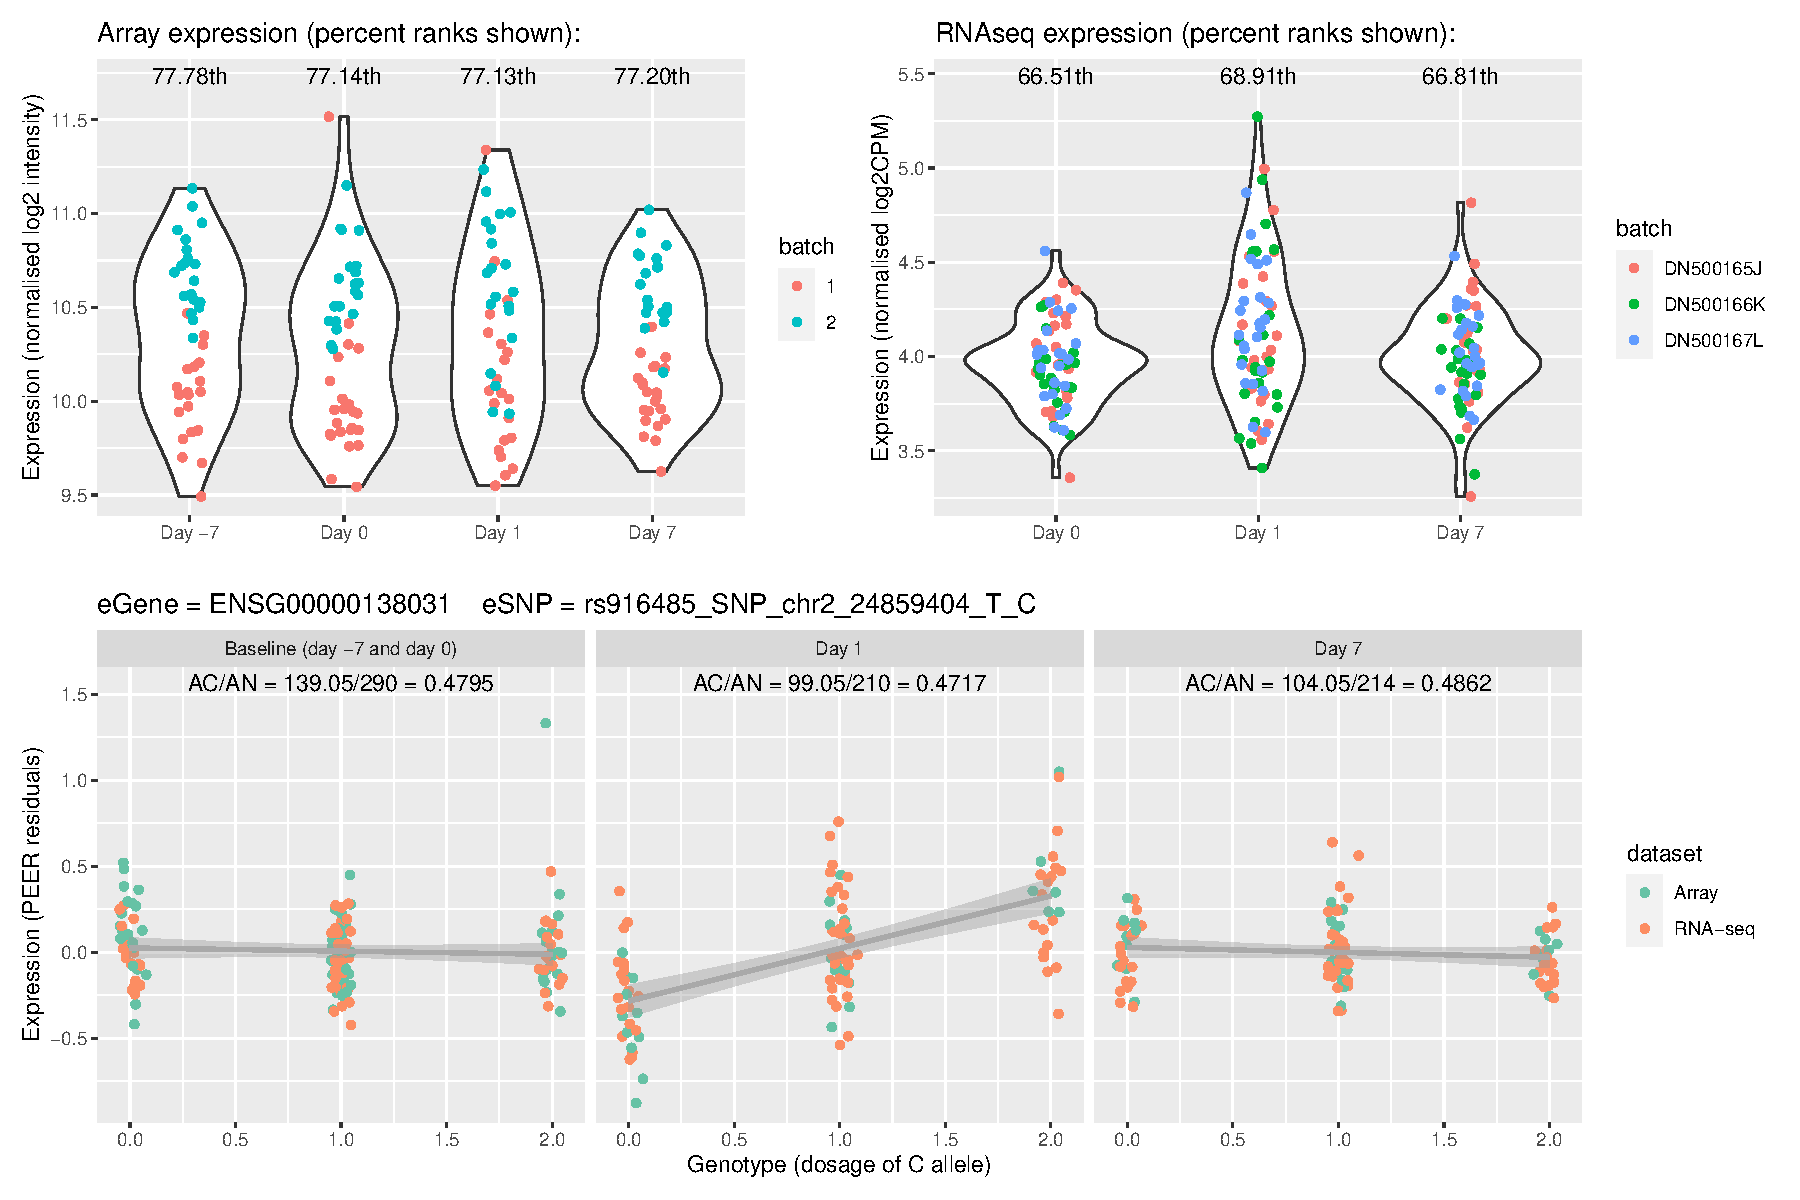
\includegraphics[width=1.0\textwidth,page=1]{mainmatter/figures/chapter_03/plot_dge_eqtl_genotypes.ENSG00000138031,rs916485_SNP_chr2_24859404_T_C.pdf}
    \caption{}
    \label{fig:hird_eQTL_ploteQTL_ADCY3}
\end{figure}

\begin{figure}
    \centering
    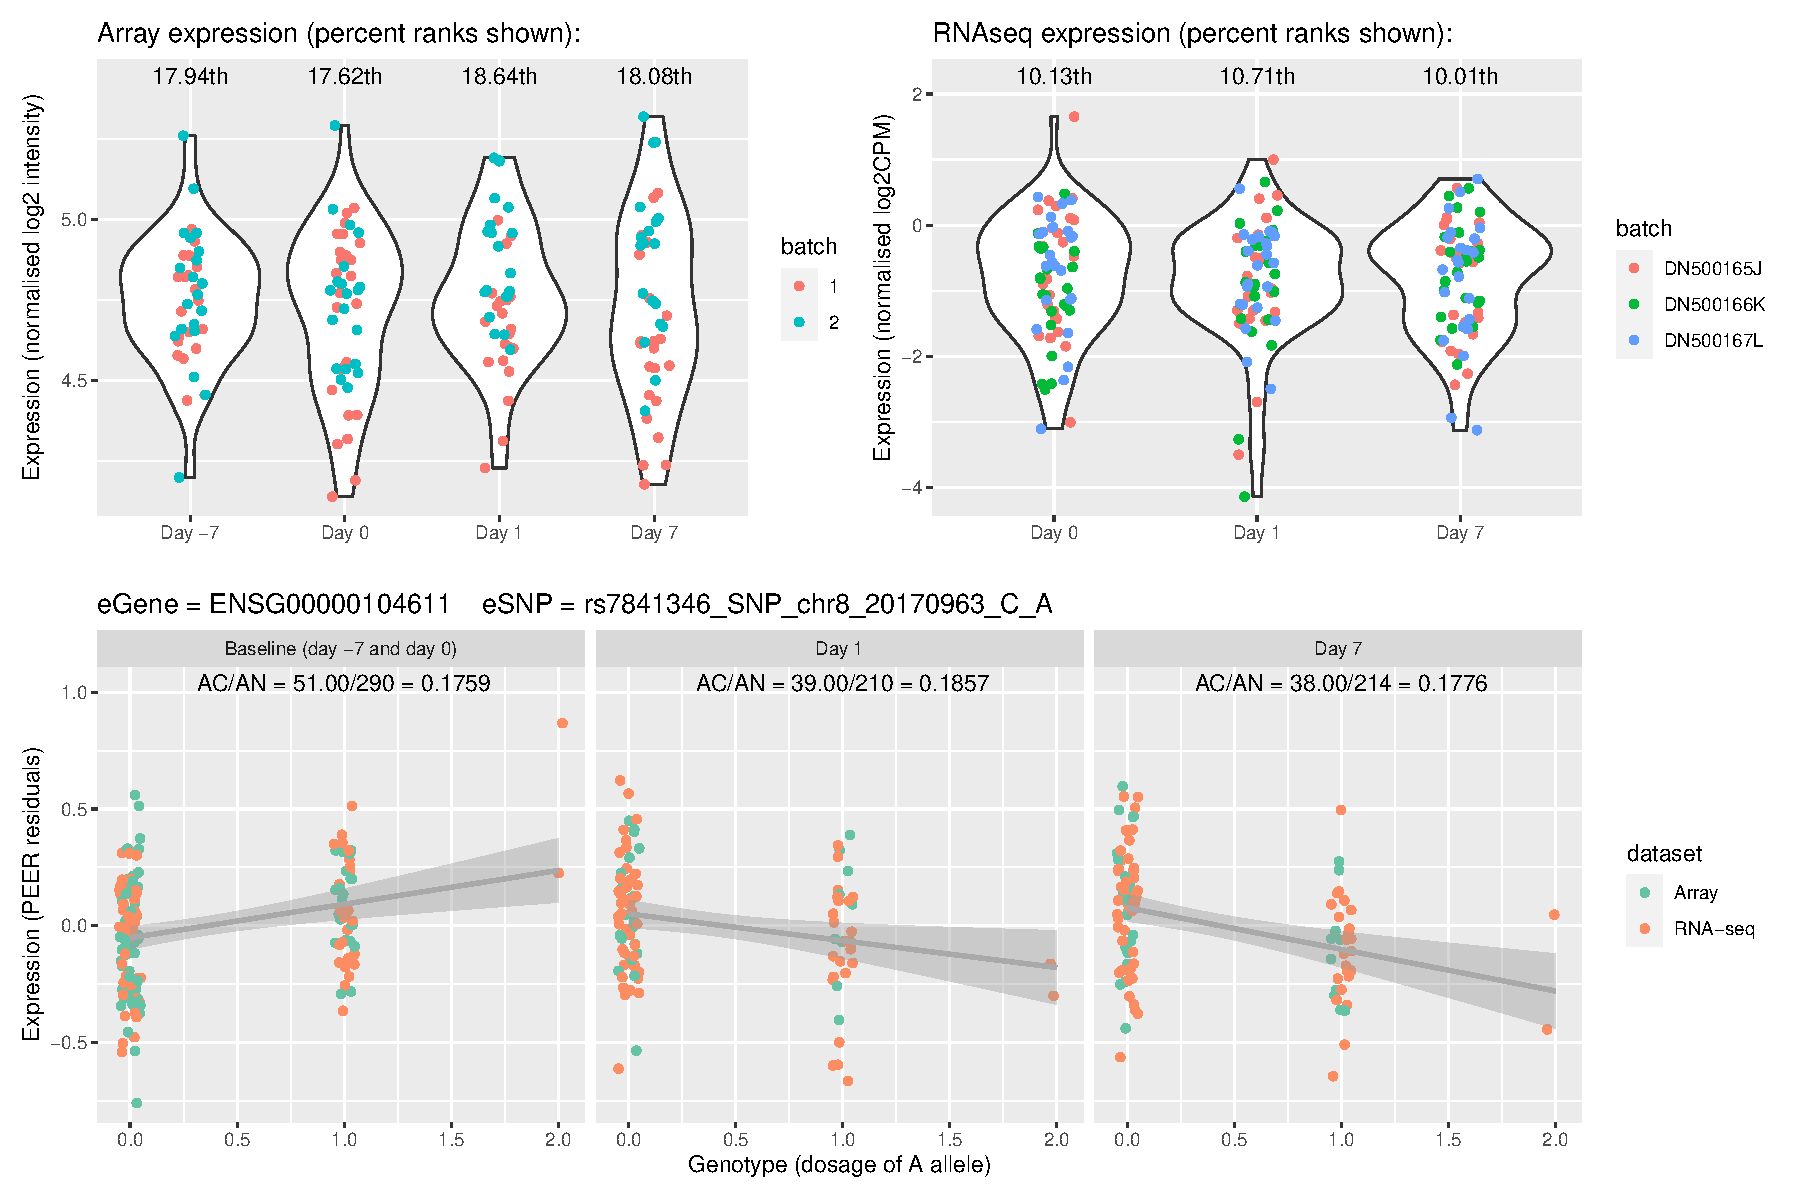
\includegraphics[width=1.0\textwidth,page=1]{mainmatter/figures/chapter_03/plot_dge_eqtl_genotypes.ENSG00000104611,rs7841346_SNP_chr8_20170963_C_A.pdf}
    \caption{}
    \label{fig:hird_eQTL_ploteQTL_SH2D4A}
\end{figure}

\subsection{Genotype by cell type interaction effects}

Given that many \glspl{reQTL} are not explained by differential expression post-vaccination, the presence of cell type-specific \gls{eQTL} effects was considered.
Standardised \software{xCell} enrichment scores were used to approximate abundance of 7 \gls{PBMC} cell types from the expression data.
\todo{move this up to model}
After pruning highly correlated cell types, scores for monocytes, \gls{NK} cells and plasma cells remained.
Within-timepoint full \gls{eQTL} models including the genotype main effect, the three cell type abundances, and three cell type-genotype interaction terms, were fit using \software{lme4qtl}, 
then compared to a nested model excluding the three interaction terms.

Significant cell type interactions were detected at 16/1154 \glspl{reQTL} (BH FDR < 0.05)
\todo{gene set enrichment for cell type interacting genes to further validate xCell score usefulness}
For \gene{ADCY3}, at day 1 post-vaccination, the full model had significantly better model fit ($chisq(3) = 26.290769$, \gls{LRT} BH FDR = \num{9.539518e-05}).
Although the genotype effect size was \num{0.255954767} (SE = \num{0.03339378}) in the nested model,
the estimate in the full model was \num{-0.007216815} (\num{0.06656115});
with the three cell type-genotype interaction term estimates being:
monocyte \num{0.212978154} (\num{0.04897962}),
\gls{NK} cells \num{-0.009195402} (\num{0.04470412}),
and plasma cells \num{0.016151511} (\num{0.06632921}).
\todo{this is probably what tables are for}
This indicates the \gls{eQTL} effect is actually driven largely by the monocyte abundance;
in the case when monocyte abundance is zero (representing an average abundance across all samples, as scores are standardised), the effect of increasing genotype dosage on \gene{ADCY3} expression is minimal.
\missingfigure{expression vs monocyte xCell score, colored by genotype}

\subsection{TODO Genotype by platform interaction effects}

% pull platform interaction in as a filter
%
% potential problems with mega discussed b4
% - platform fx
% - Using a fixed effect assumes mean diff between rnaseq and array and forces the slope to the average.
% - lme4qtl interactions with bonferroni
- Perhaps using platform specific effects as a filter for reQTLs.

\subsection{TODO Colocalisation of reQTLs with known \textit{in vitro} condition-specific immune eQTLs}

% TODO
% Choice of method;
% See coloc_comparisons in notes for a summary
% Coloc and assumptions; Hypercoloc and assumptions
\begin{outline}

% rs916485_SNP_chr2_24859404_T_C
\1 In a 500 Mb window around the lead \gene{ADCY3} variant rs916485, \software{hyprcoloc} to colocalise with existing datasets and fine map.

\1 Day 1 HIRD colocs with BLUEPRINT and Fairfax monocytes (both stim and non stim), but not with Quach (\autoref{fig:hird_eQTL_coloc_ADCY3}).
\2 Biases from ethnicity-derived differences in LD?
\2 Also, priors need tuning?

% fine mapped to 2_24874775_A_G, nearest gene (45,064 bp downstream to canonical TSS): ADCY3 TSS is at 24919839, rev strand
\1 Fine mapped to rs13407914 (PP = 1), an intronic variant 45064 bp downstream of the TSS.

% note in 2019-06-17_team_meeting.pptx, originally was rs10185143
\todo{FYI the IBD/T cell coloc fine maps to chr2:24935139 T C (rs713586) with PP=1}

\end{outline}

\begin{figure}
    \centering
    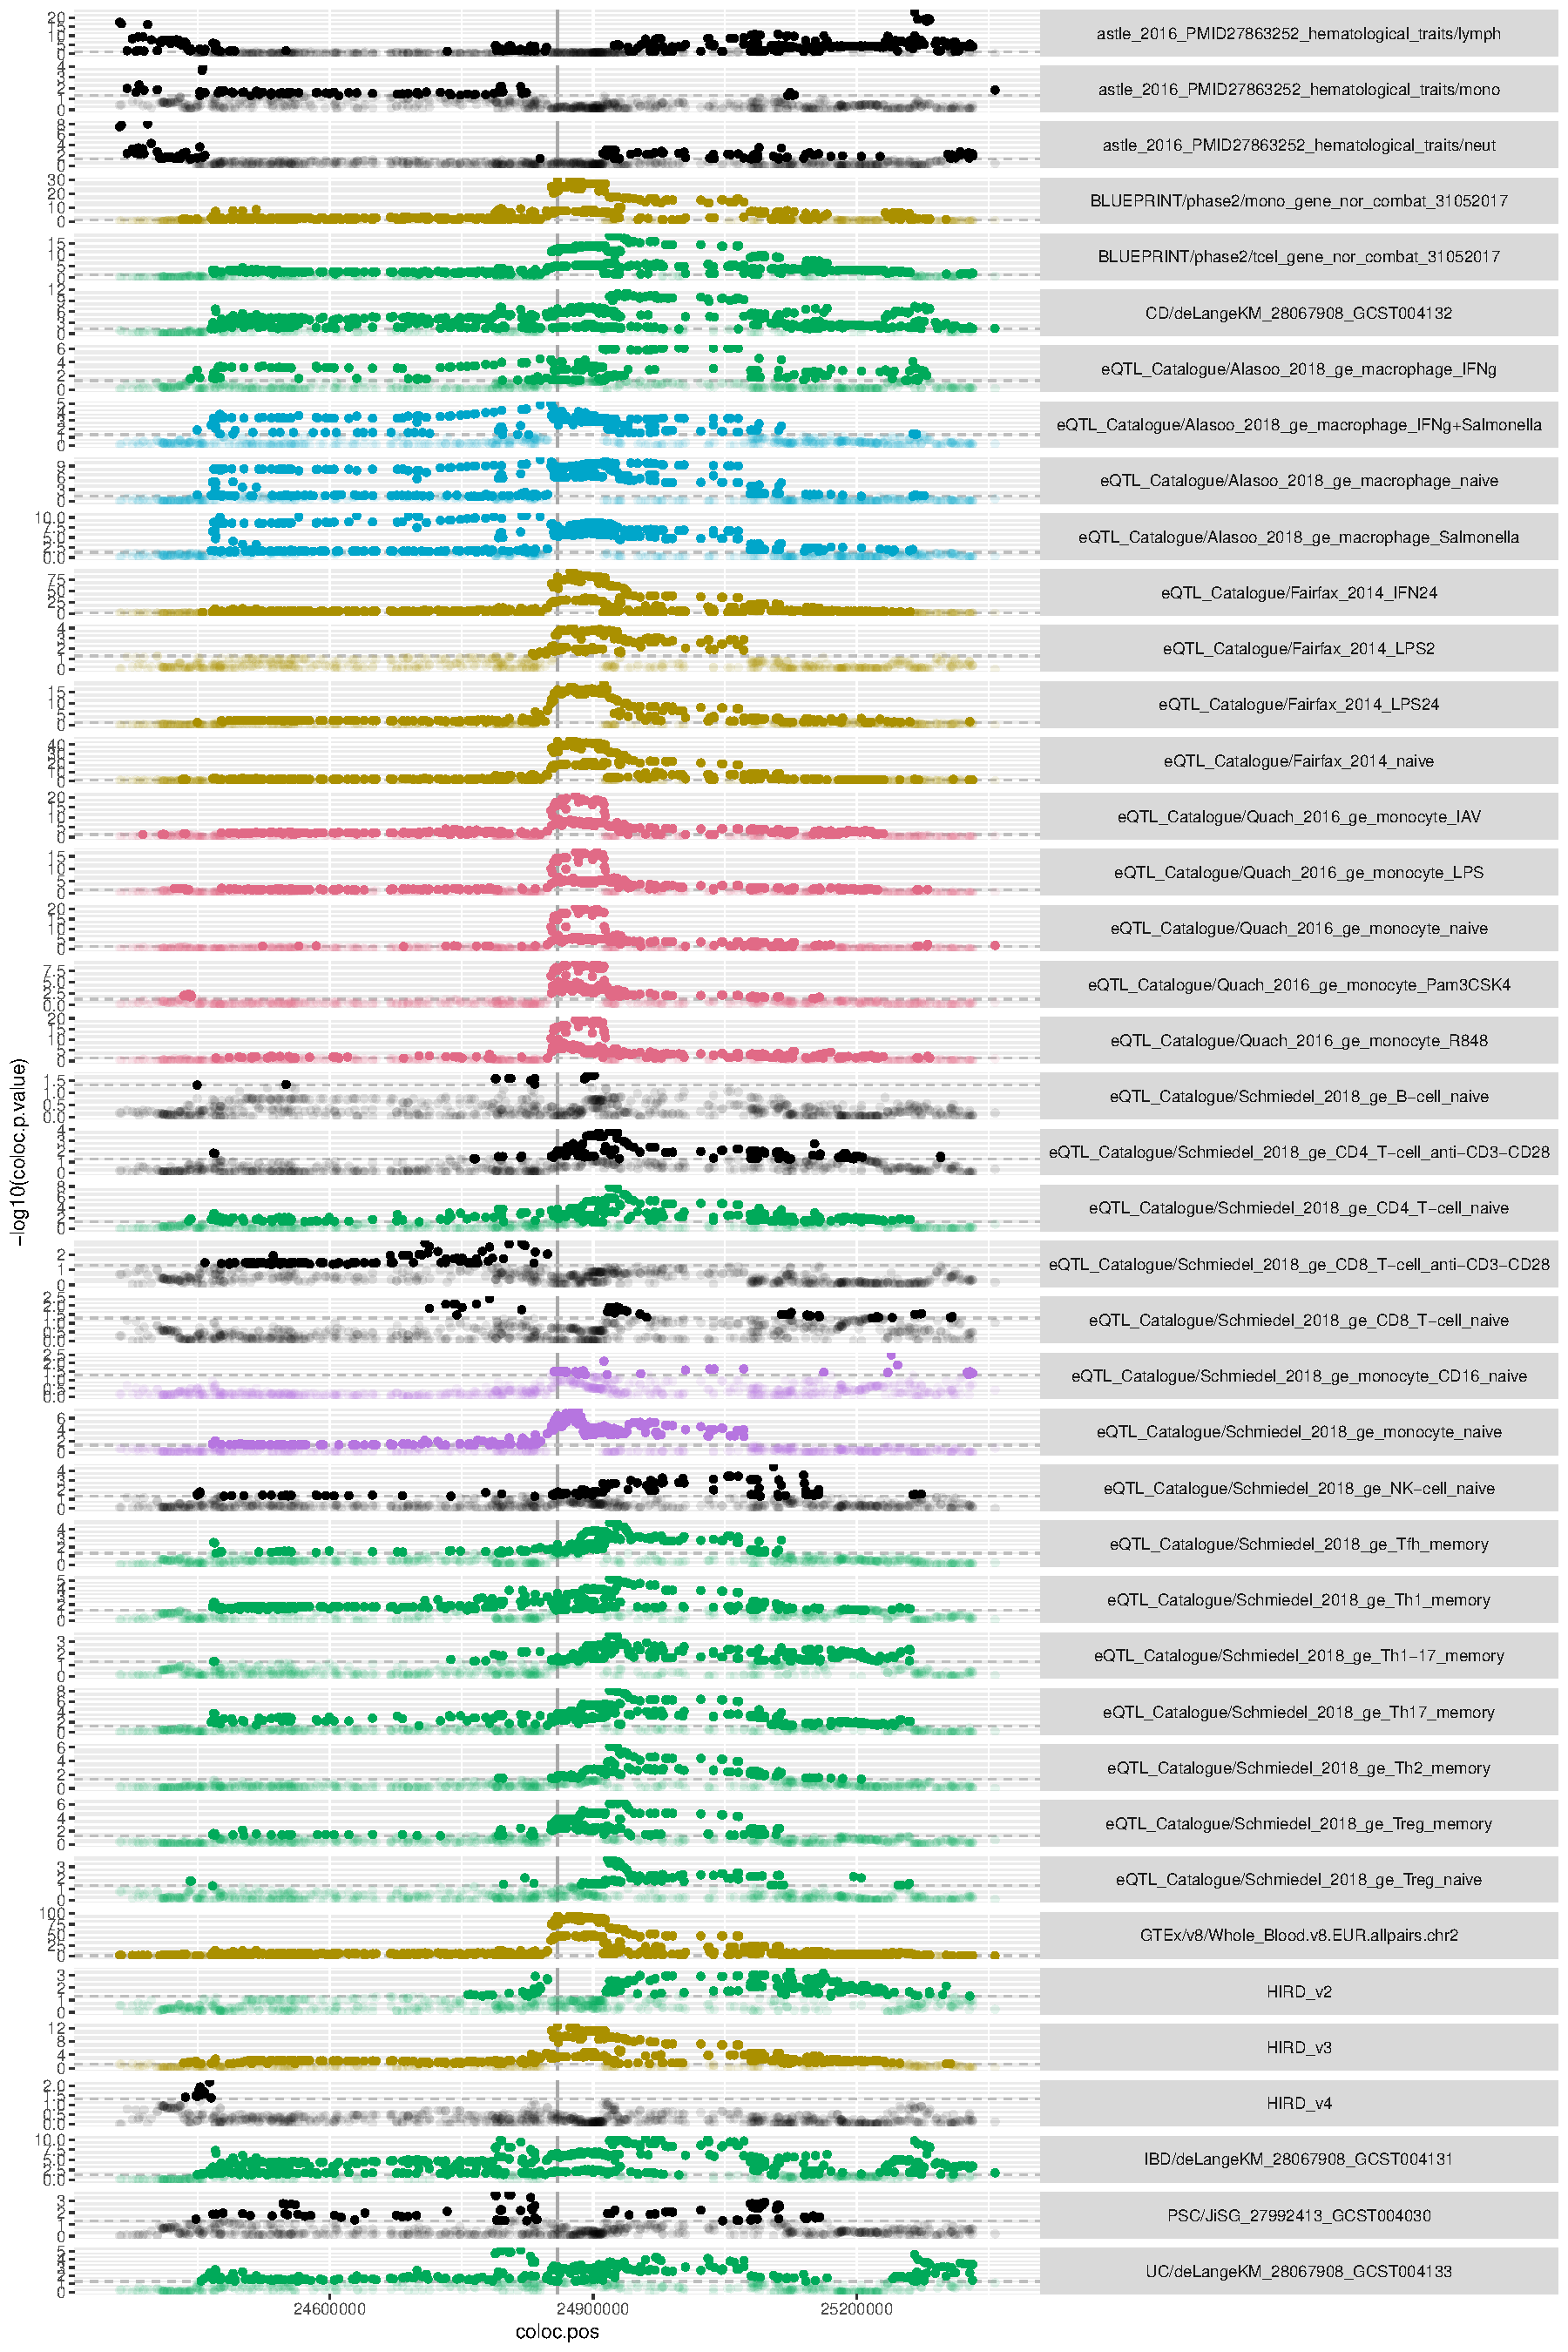
\includegraphics[width=1.0\textwidth,page=1]{mainmatter/figures/chapter_03/perform_coloc.locusPlot.gene_ENSG00000138031.pdf}
    \caption{}
    \label{fig:hird_eQTL_coloc_ADCY3}
\end{figure}

\section{Discussion}

% TODO: here
Overall summary

more reqtls at d1, expected, but no
Given the large changes in expression, detect context-specific fx.

% parameters of innate cells were more strongly controlled by genetic variation than were those of adaptive cells,
% "https://www.nature.com/articles/s41590-018-0049-7#Abs1"

How much sharing vs expected?
In the multi-tissue paradigm: cite the GTEx U curve

op effects may be more common
% https://www.nature.com/articles/s41431-019-0468-4#Sec9
oppposite effect has greater power to detect


Confounded by changes in immune cell proportions in bulk PBMCs;
as cell type -> E, but also modified G -> E
how good is our deconv? stim at day 1
Note, the use of gene signatures for deconv
    in stimulated samples
    does not distinguish upreg from prolif either
    if expression goes up, the method will detect more of the signature
    i.e. it may correct away some signal of upregulation

computational reasons
only test top snp, miss some 
assume that main effect is signif 
lme4qtl was not scalable

Confounding by multiple causal variants?;
No conditional eQTL analysis to disentangle conditional effects;

miss some reQTLs
Are re qtls more likely to be distal and secondary?



e.g. ct specific
ACDY3 talk
The strongest \gls{reQTL} detected at day 1 was \gene{ADCY3}, 
effect probs due to large mono abundance at d1
or correlated

franco, but
- an example of d1 reQTL at adcy3


and in:
whole blood
% (A) ADCY3, (B) DNAAF1 and (C) ZNF517):
% before and after stimulation with M. leprae sonicate in whole blood cells.
% https://journals.plos.org/plosgenetics/article?id=10.1371/journal.pgen.1006952
and in: 
caliskan

and in High-throughput allele-specific expression across 250 environmental conditions
% https://www.ncbi.nlm.nih.gov/pmc/articles/PMC5131815/

% PBMCs Rhinovirus in vitro
% https://www.ncbi.nlm.nih.gov/pmc/articles/PMC4395341/
% In fact, six (SLFN5, ARL5B, SPTLC2, IRF5, ADCY3, CCDC146) of the 38 genes
% implicated in our reQTL mapping were also identified in a recent reQTL mapping
% study for Escherichia coli lipopolysaccharide, influenza, and interferon-β in
% dendritic cells [35].
%
% Additionally, our results imply that the SNPs residing in STAT2 binding sites
% are more likely to be the causal SNP in the reQTL loci of EXOSC9, SLFN5, PRR24,
% OAS1, and ARL5B. In fact, causality of the reQTL of SLFN5 gene, rs11080327, was
% recently demonstrated by luciferase reporter assays [35].

% 2017
% whole blood
% M. leprae in vitro
% https://www.ncbi.nlm.nih.gov/pmc/articles/PMC5565194/
% Examples of three reQTL among genes found only in M. leprae sonicate stimulated
% cells or non-stimulated cells. For each gene ((A) ADCY3, (B) DNAAF1 and (C)
% ZNF517): the left panel corresponds to the expression of the gene in
% non-stimulated cells while the right panel depicts expression of the gene in
% stimulated cells. The gene identity is indicated above each pair of graphs. The
% gene expression level in log2 scale (y-axis) is plotted for each genotype
% (x-axis). Of note, reQTL for the ADCY3 and DNAAF1 genes have been found by
% other studies using distinct pathogens or molecules as stimuli, while the reQTL
% for ZNF517 is a newly identified reQTL [21, 22, 24, 26]. ADCY3 is among the
% most upregulated genes after stimulation with M. leprae antigens and has been
% identified as part of the T1R gene set signature identified by Orlova et al.
% [32]. The reQTL for DNAAF1 displays the strongest P value among the reQTL we
% identified.

so likely broad innate response, rather than vacc specific



Biggest question remains, why are reQTLs reQTLs

dge eqtl overlap poor?
average no dge, but dge by genotypes
what other mechs?
can be indep
like davenport, we observe little overlap

attempt to addres by coloc
% Colocalisation with known associations [...]
% Colocalisation is used to understand the molecular basis of GWAS associations (of a variety of human disease traits) (Giambartolome, 2014) [...]
% Here the inverse: coloc is used to understand the biological relevance of observed expression variation.
can miss

% fu mechs
TFs are tissue specific
% https://www.biorxiv.org/content/biorxiv/early/2019/10/06/785584.full.pdf

davenport etc. demonstrated tfs

% tf review
% https://www.cell.com/cell/pdf/S0092-8674(18)30106-5.pdf

introns can be TF bound
% https://journals.plos.org/plosone/article?id=10.1371/journal.pone.0046784

% rs13407913
% cursory scan: http://54.245.180.226/php_file/multiple.php?ID=rs13407913
% SP1 is monocyte specific https://europepmc.org/article/med/28008225
and upreg at d1

need more principaled scan



Unclear connection to vaccine biology e.g. what genesets/pathways/cell types are driving the observed transcriptomic and eQTL response?;
big lim: sample size: unable to leverage Ab data for mediation analysis
misses a main advantage of in vivo design

Need GWAS 

franco: It must be said, overlap is not rigorous
    they recog Formal Mediation analysis required


